\documentclass[twoside,11pt]{article}

\usepackage{algorithm}
\usepackage{algpseudocode}
\usepackage{jmlr2e}
\usepackage{amsmath}
\usepackage{booktabs}
\usepackage{array}
\usepackage{lastpage}
\usepackage{xspace}
\urlstyle{tt}

\newcommand{\R}{\mathbb{R}}
\newcommand{\argmin}{\mathop{\mathrm{argmin}}}
\newcommand{\norm}[1]{\left\lVert #1 \right\rVert}
\newcommand{\fuserplus}{\texttt{fuserplus}\xspace}
\DeclareMathOperator{\clip}{clip}

\jmlrheading{1}{2026}{1-\pageref{LastPage}}{4/26}{--}{26-0000}{Agyapong}
\ShortHeadings{Sparse-Graph Solvers for Grouped Fused Regression}{Agyapong}
\firstpageno{1}

\begin{document}

\title{Sparse-Graph Representations for Scalable Grouped Fused Lasso Regression}

\author{\name Daniel Agyapong \email da2343@nau.edu \\
       \addr School of Informatics, Computing, and Cyber Systems\\
       Northern Arizona University\\
       Flagstaff, AZ, USA
       \AND
       \name Michael Gowanlock \\
       \addr School of Informatics, Computing, and Cyber Systems\\
       Northern Arizona University\\
       Flagstaff, AZ, USA
       \AND
       \name Jane Marks \\
       \addr Department of Biological Sciences\\
       Northern Arizona University\\
       Flagstaff, AZ, USA
       \AND
       \name Toby Dylan Hocking \\
       \addr D\'epartement d'informatique\\
       Universit\'e de Sherbrooke\\
       Sherbrooke, QC, Canada}

\editor{}

\maketitle

\begin{abstract}
Although the statistical graph in grouped fused regression is often sparse, standard implementations still materialize full pairwise fusion operators or augmented designs, making the computational representation much denser than the model.
We propose sparse-graph representations for grouped fused regression that preserve the graph edge set directly in the optimizer.
For L1 fusion, an active-edge operator evaluates the same smoothed proximal-gradient fusion term using only nonzero graph edges.
For L2 fusion, an active-edge augmented-design construction emits sparse triplets only for the modeled edges before solving the regularized path.
These constructions preserve the main objective in the exact L1 and L2 cases while reducing the dominant fusion representation from full-pairwise graph construction to edge-linear construction.
Our empirical comparisons hold the optimizer family fixed relative to reference grouped fused-regression solvers, so that the measured differences isolate graph representation rather than changes in optimization architecture.
We also analyze a chain approximation L1 solver which trades graph fidelity for additional efficiency thereby slightly reducing accuracy.
For the exact L1 and L2 solvers, the active-edge representation changes the dominant fusion-side construction from all-pairs dependence on \(\binom{k}{2}\) candidate group pairs to edge-linear dependence on the \(m\) modeled graph edges.
The chain approximation L1 solver further reduces the represented fusion graph to \(k-1\) edges, so as to solve an approximate chain-fusion problem.
On public grouped-regression datasets, we illustrate that the exact active-edge methods preserve predictive accuracy while reducing the dominant fusion-side representation cost from dependence on all \(\binom{k}{2}\) group pairs to dependence on the \(m\) active graph edges.
The largest practical efficiency gains occur for sparse graphs with many groups (above 100).
% The algorithms are available in the open-source R implementation at
% \href{https://github.com/EngineerDanny/fuserplus}{https://github.com/EngineerDanny/fuserplus}.
\end{abstract}

\begin{keywords}
  fused lasso, grouped regression, sparse graphs, structured sparsity,
  first-order optimization
\end{keywords}

\section{Introduction}
Many regression problems contain a natural grouping variable such as patients may belong to disease subtypes, schools to districts or countries to continents \citep{gelman2007data}.
Fitting a separate model in each group ignores shared signal, whereas fitting one global model forces all groups to share the same coefficients.
Grouped fused regression addresses this middle ground by estimating one coefficient vector per group and penalizing differences between coefficient vectors along a graph of group relationships.

Let $X_g \in \R^{n_g \times p}$ and $y_g \in \R^{n_g}$ denote the data for group $g$, and let $\beta_g \in \R^p$ be that group's linear coefficient vector. 
For a graph $G=(V,E)$ over $k$ groups with nonnegative edge weights $w_{gh}$, the estimators considered in this paper have the form
\begin{equation}
\label{eq:model}
  \min_{\beta_1,\ldots,\beta_k}
  \sum_{g=1}^{k} \frac{1}{2 n_g} \norm{y_g - X_g \beta_g}_2^2
  + \lambda \sum_{g=1}^{k} \norm{\beta_g}_1
  + \gamma \sum_{(g,h)\in E} w_{gh} \Omega(\beta_g-\beta_h).
\end{equation}

For the L1 fused model, $\Omega(u)=\norm{u}_1$; for the L2 fused model, $\Omega(u)=\frac{1}{2}\norm{u}_2^2$ after the standard augmented-design reformulation. 
This formulation is a direct descendant of the lasso, fused lasso, grouped and elastic-net regularization, graph-structured fused optimization, and subgroup regression models. 
The L1 solver uses the standard Nesterov smoothing strategy for nonsmooth penalties \citep{nesterov2005smooth}.
The central computational issue is that the model may use only a sparse set of graph edges, while the solver may still construct fusion terms for all possible pairs of groups.
A complete graph has \(k(k-1)/2\) edges, but practical graphs are frequently chains \citep{hoefling2010path}, trees \citep{padilla2018dfs}, nearest-neighbor graphs \citep{padilla2020knn}, or sparse networks informed by prior knowledge \citep{hallac2015network}.
If the objective is defined on only $m$ active edges, a solver that builds all pairwise fusion constraints and then uses zero weights for inactive edges changes the computational scaling of the problem without changing its statistical content. 
This matters especially as \(k\) grows. 
The modeling graph may be sparse, but the reference representation still scales with all \(\binom{k}{2}\) group pairs.

The paper therefore evaluates graph representation as the primary algorithmic variable, while keeping the underlying optimizer family fixed.
For L1 fusion, both the reference solver and the exact active-edge solver use the same smoothed proximal-gradient framework. 
For L2 fusion, both the reference solver and the active-edge solver use the same augmented-design reduction before fitting the regularized path.
Alternative methods such as ADMM-based solvers \citep{boyd2011admm,hallac2015network} and split-Bregman solvers \citep{ye2011split} are important for nonsmooth fused penalties, but they change the optimization architecture and introduce additional tuning and implementation choices.
The comparisons here are designed to isolate the effect of preserving the sparse graph inside the existing grouped fused-regression optimization framework.
The contribution of this paper is an algorithmic representation of grouped fused regression that makes the sparse graph a first-class object in the optimizer. 
Instead of constructing all possible group-pair fusion terms and encoding graph sparsity through zero weights, the proposed representations operate directly on the modeled graph edges. 
This principle yields exact active-edge L1 and L2 reformulations, and also motivates approximate high-efficiency solvers when additional graph reduction is acceptable.

The main contributions are:
\begin{itemize}
\item a sparse-graph representation principle for grouped fused regression solvers;
\item exact active-edge L1 and L2 reformulations that preserve the reference objective while avoiding zero-weight all-pair construction;
\item complexity reductions that replace fusion-side dependence on all \(\binom{k}{2}\) group pairs with dependence on the \(m\) modeled graph edges;
\item a clear separation between exact sparse-graph solvers and approximate chain variants that reduce the represented graph to \(k-1\) edges;
\item a controlled empirical design that keeps the optimizer family fixed and isolates the effect of graph representation; and
\item empirical comparisons showing that active-edge construction preserves predictive accuracy while reducing runtime and memory on public grouped-regression benchmarks.
\end{itemize}

The remainder of the paper is organized as follows. 
Section~2 reviews fused and graph-structured regression methods, together with related optimization approaches. 
Section~3 defines the grouped fused-regression model and the full-pairwise computations used as references. 
Section~4 presents the active-edge L1, the active-edge L2 augmented-design construction, and the chain approximation. 
Section~5 describes the benchmark protocol, datasets, and compared methods. Section~6 reports accuracy, timing, memory, and  efficiency results. 
Section~7 discusses implications, limitations, and implementation guidance, and Section~8 summarizes reproducibility materials.


\section{Related Work}

The fused lasso extends the lasso by combining sparsity with penalties on ordered coefficient differences \citep{tibshirani1996lasso,tibshirani2005fused}.
Grouped fused regression adapts this idea to grouped data by estimating one coefficient vector per group and penalizing differences between coefficient vectors along a graph of group relationships.
This places grouped fused regression in a broader family of structured regularizers, including the elastic net, group lasso, generalized lasso, and graph trend filtering \citep{zou2005elastic,yuan2006group,tibshirani2011genlasso,wang2016graphtf}.
Specialized algorithms for one-dimensional signal approximation, including path algorithms for the fused lasso signal approximator, exploit the ordered chain structure of that problem \citep{hoefling2010path}. 
Split-Bregman and ADMM methods provide another important optimization line for nonsmooth fused penalties \citep{ye2011split,boyd2011admm}. 
General graph fusion is more flexible but computationally harder because the penalty couples many coefficient blocks.

It is useful to separate three forms of fusion that are discussed under related fused-lasso terminology. 
In the classic fused lasso, the ordered objects being fused are usually variables, coordinates, or signal locations.
For a single regression vector, this means penalizing adjacent coefficient differences such as $|\beta_{j+1}-\beta_j|$. 
In graph-guided multi-task learning, the fused objects are tasks, often corresponding to related responses or prediction problems. 
In grouped fused regression, the fused objects are groups of observations in one regression problem. 
The model estimates a coefficient matrix $B\in\R^{p\times k}$, with one column for each group. 
The fusion graph is on the groups, and an edge $(g,h)$ penalizes the difference between the two coefficient vectors $B_g$ and $B_h$. 
The focus of this paper is entirely on fusion between groups, not fusion between variables or responses.

Figure~\ref{fig:fusion-matrix-concepts} illustrates these distinctions.
Classic variable fusion acts within a single ordered coefficient vector, as in the fused lasso \citep{tibshirani2005fused}. 
Multi-task fusion encourages sharing across columns of a coefficient matrix, where the columns correspond
to responses or tasks \citep{chen2010graph,chen2012smoothing}. 
Grouped fused regression also encourages sharing across columns, but the columns are groups from one grouped regression problem with common predictors and a common response \citep{dondelinger2020joint}. 
This is why graph-guided multi-task learning is related but not identical to the problem studied here.

\begin{figure}[t]
  \centering
  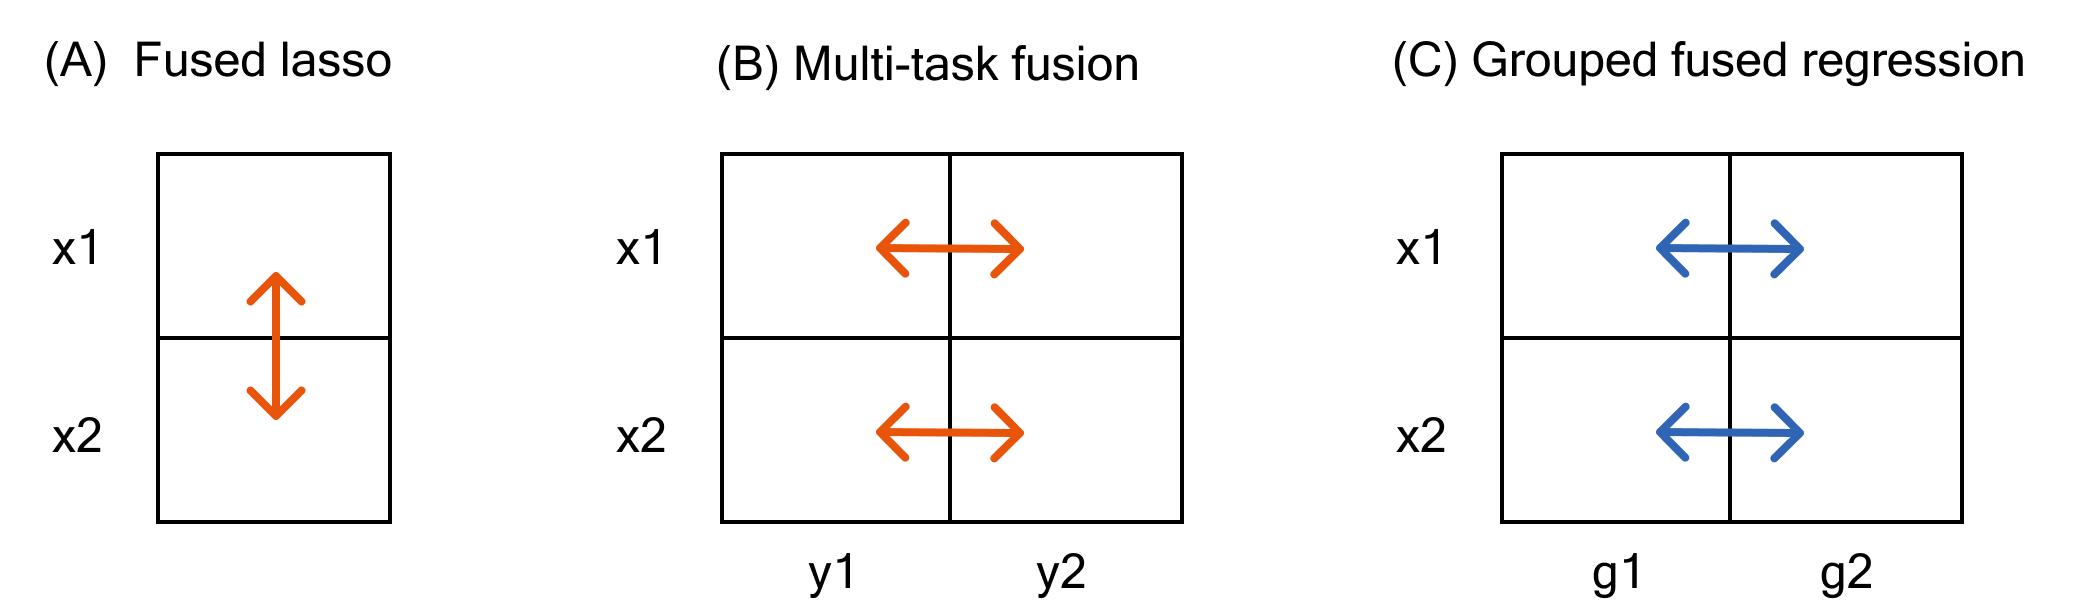
\includegraphics[width=.95\textwidth]{figures/concept_fusion.png}
\caption{Three fusion forms shown as coefficient matrix schematics. 
Rows labeled $x_1$ and $x_2$ denote predictors.
In Panel B, columns $y_1$ and $y_2$ denote related responses or tasks. 
In Panel C, columns $g_1$ and $g_2$ denote groups of observations. 
Links indicate which objects are coupled by the fusion penalty. 
Panel A shows fused lasso penalties on ordered coefficients \citep{tibshirani2005fused}. 
Panel B shows graph-guided multi-task fusion across related responses or tasks \citep{chen2010graph,chen2012smoothing}. 
Panel C shows grouped fused regression, where the fusion graph is placed on groups of observations
\citep{dondelinger2020joint}. 
This grouped fused regression, is what we focus on in this paper.}
  \label{fig:fusion-matrix-concepts}
\end{figure}

Graph-structured multi-task regression extended these ideas to arbitrary task graphs and developed smoothed proximal-gradient methods for the general fused lasso \citep{chen2010graph,chen2012smoothing}. 
Related multi-task and scientific applications use graph-guided fusion for eQTL mapping, additive modeling and gene regulatory network inference \citep{chen2012twograph,petersen2016flam,omranian2016gene}.
Network lasso methods \citep{hallac2015network}, graph trend filtering, Depth First Search (DFS) fused lasso denoising \citep{tansey2018dfs}, and k-nearest-neighbor fused lasso estimators \citep{padilla2020adaptive} further emphasize that the graph itself is part of the modeling problem. 
The crucial idea is that the graph may come from prior knowledge, distances between groups, or other data-driven structure.

The present work focuses on how grouped fused regression objectives should be represented and solved especially when the graph is sparse. 
The graph is part of the modeling assumption, and a dense all-pairs representation discards that assumption at the computational layer. 
The active-edge constructions proposed restore the intended edge-level representation while preserving the objective in the exact L1 and L2 cases.

Table~\ref{tab:literature-comparison} summarizes the existing methodological literature. 
The comparison is organized around modeling and optimization ideas. 
The novel contribution of this paper is an active-edge representation that preserves a sparse graph inside the existing grouped fused-regression objective. 
In this view, the closest statistical existing literatures are the joint-lasso/grouped fused-regression formulation of \citet{dondelinger2020joint} and the graph-guided multitask learning and smoothed proximal-gradient methods for general fused penalties \citep{chen2010graph,chen2012smoothing}. 
The role of the present work is to isolate the representation question. 
This implies that when the graph is sparse, the optimization data structures should scale with the active edge set rather than with all possible group pairs.

\begin{table}[t]
\centering
\scriptsize
\caption{Existing methodological literature and distinctions from the present work.
The paper builds on graph-fused regression and smoothed first-order optimization, but focuses on preserving sparse edge sets in the solver representation while holding the objective and optimizer family fixed.}
\label{tab:literature-comparison}
{\setlength{\tabcolsep}{3pt}
\renewcommand{\arraystretch}{1.5}
\begin{tabular}{@{}>{\raggedright\arraybackslash}p{0.24\textwidth}
>{\raggedright\arraybackslash}p{0.33\textwidth}
>{\raggedright\arraybackslash}p{0.34\textwidth}@{}}
\toprule
Literature & Main idea & Distinction from this paper \\
\midrule
Lasso and fused lasso \citep{tibshirani1996lasso,tibshirani2005fused} &
Combines sparsity with penalties on adjacent coefficient differences. &
Introduces the core sparsity and fusion penalties, while this paper studies how to represent sparse fusion graphs efficiently in grouped fused-regression. \\
Graph-guided multitask regression \citep{chen2010graph,chen2012smoothing,chen2012twograph} &
Uses task graphs and smoothed proximal-gradient methods for general fused multitask penalties. &
This paper uses related graph-fusion ideas to target grouped regression instead of general multitask learning. \\
Generalized lasso and graph trend filtering \citep{tibshirani2011genlasso,wang2016graphtf} &
Uses linear operators or graph differences to encode structured variation. &
Provides a broad operator framework, whereas this paper focuses on preserving sparse graph edges inside grouped fused-regression solvers. \\
Split-Bregman and ADMM approaches \citep{ye2011split,boyd2011admm} &
Introduce auxiliary variables for nonsmooth penalties and solve alternating subproblems. &
The comparisons in this paper keep the smoothed first-order optimization framework fixed to isolate the effect of graph representation. \\
Network lasso and graph-based fusion \citep{hallac2015network} &
Penalizes graph-edge differences to cluster or share information over networks. &
Uses graph-edge penalties to share information over networks, but studies a different objective and optimization framework from the grouped fused-regression in this paper. \\
Joint lasso for subgroup regression \citep{dondelinger2020joint} &
Estimates grouped regressions with sparsity and fusion across groups. &
Closest statistical predecessor and reference used in this paper. This paper preserves its objective while replacing all-pair graph construction with active-edge construction. \\
Graph decomposition for graph-fused lasso \citep{yu2025graphdecomp} &
Uses graph decomposition to build a faster ADMM algorithm for graph-fused lasso on general graphs. &
Changes the ADMM decomposition and optimizer architecture; this paper keeps the smoothed L1 and augmented-design L2 solver families fixed to measure representation effects. \\
\bottomrule
\end{tabular}
}
\end{table}


\begin{figure}[t]
  \centering
  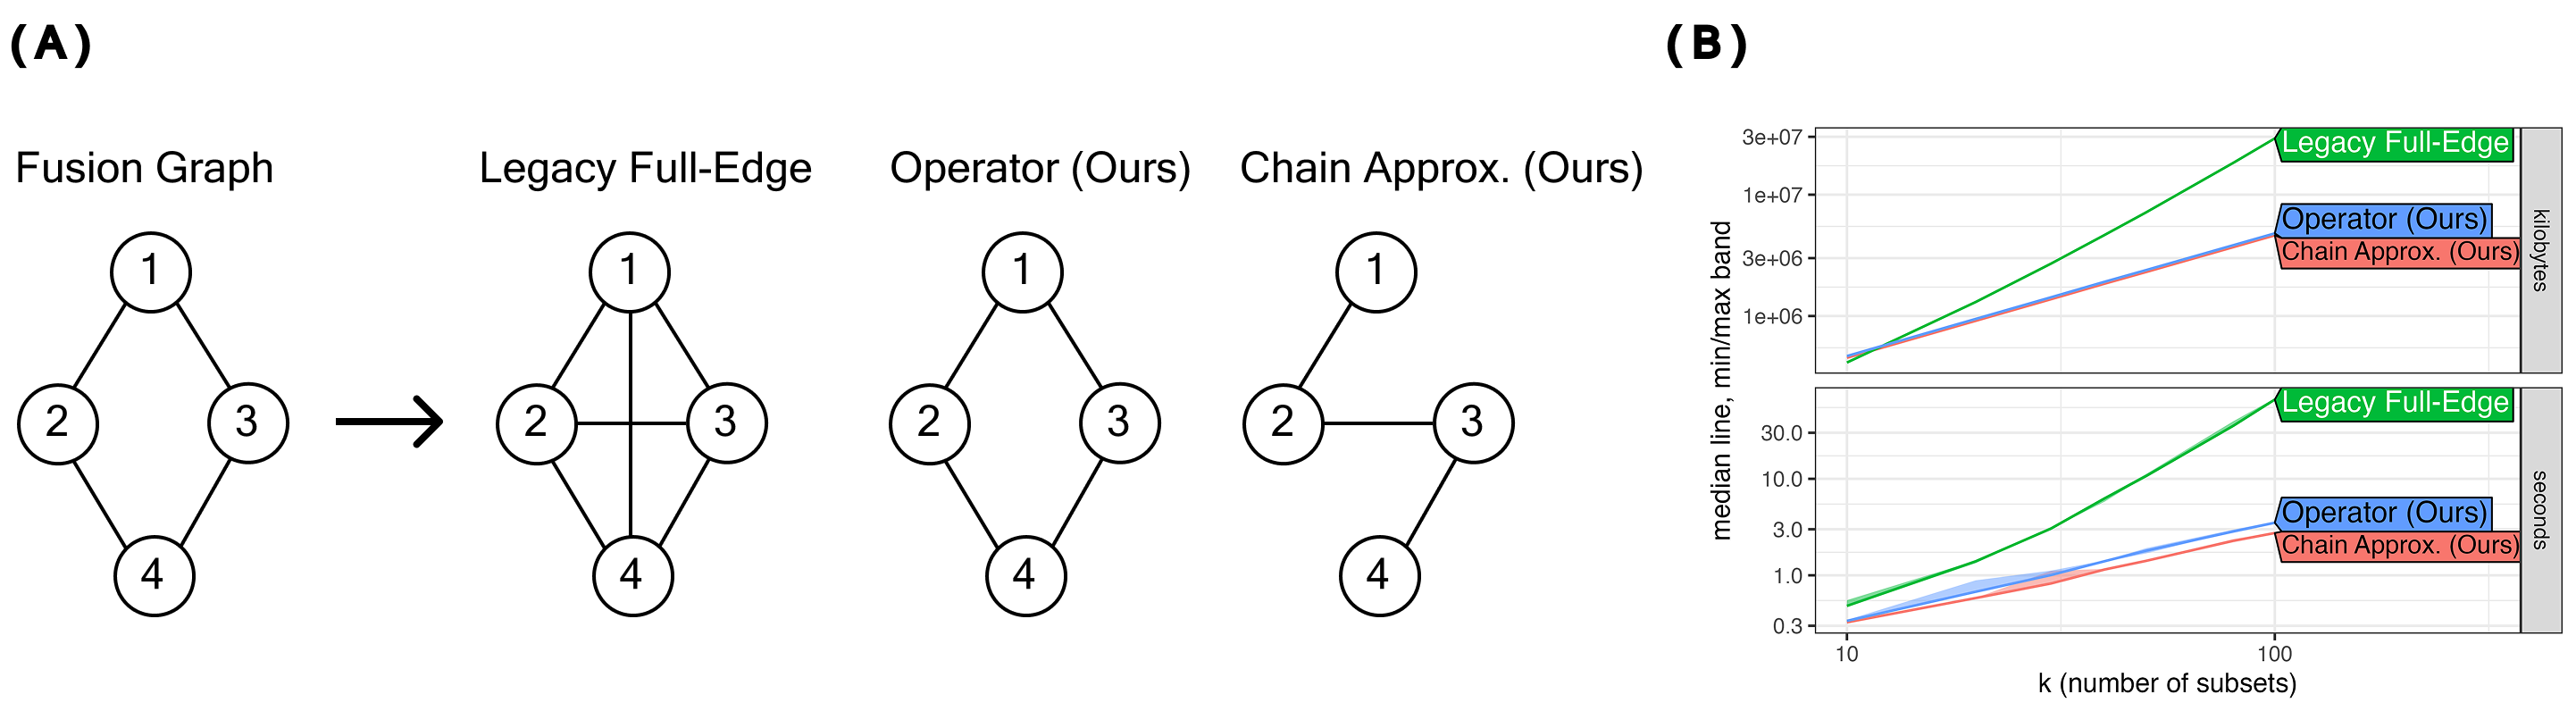
\includegraphics[width=1\textwidth]{figures/concept1.png}
  \caption{Conceptual overview of L1 sparse-graph fusion. 
  A: Fusion graph construction. 
  The reference full-edge construction associated with \citet{dondelinger2020joint} forms a combined constraint matrix over all group pairs, while the active-edge operator works directly on the sparse graph. 
  The chain approximation replaces the modeled edge set with a chain before fitting.
  B: Asymptotic complexity. 
  The synthetic example uses $p=120$ features and 35 training observations per group. 
  Thus, when the number of groups is $k=100$, the training set has $n=3500$ observations.
  The rest of the hyper-parameters are fixed.
  For the sparse chain graph, where $m$ is the number of fusion edges ($m=k-1$), the active-edge representation changes the dominant fusion cost from $O(pk^3)$ to $O(pm)$.
  }
  \label{fig:concept-l1}
\end{figure}

\section{Grouped Fused Regression and Graph Computation}
Figures~\ref{fig:concept-l1} and~\ref{fig:concept-l2} summarize the main computational distinction between the reference fused-regression representation and the sparse-graph representation. 
In both cases, the statistical model is defined by a graph on the $k$ groups, with an absolute edge weight indicating how strongly two subgroup coefficient vectors should be encouraged to agree. 
The reference construction first expands this modeling graph into a dense algebraic object over many group pairs. 
That expansion is benign for small $k$, but it becomes the dominant cost when the intended graph is sparse, because computation is then driven by the number of possible group pairs rather than by the number of modeled edges.

Figure~\ref{fig:concept-l1} describes the L1 fusion case. 
Panel A begins with the intended fusion graph. 
Nodes are regression groups and each drawn edge marks a coefficient difference penalized by the model. 
The reference full-edge construction expands that graph into an all-pairs layout for the combined L1 constraint matrix. 
In the four-group concept, it introduces pair slots that are absent from the modeled graph. 
The exact active-edge operator keeps the original graph and evaluates the nonsmooth fusion penalty only along its $m$ nonzero edges. 
The chain approximation makes a different tradeoff by replacing the original edge set with a chain before fitting. 
Panel B then shows the computational consequence. 
The active-edge L1 representation avoids the all-pairs constraint matrix, so fusion-side scaling depends entirely on the graph edges rather than powers of $k$.

Figure~\ref{fig:concept-l2} gives the analogous picture for L2 fusion.
In the quadratic case, fusion can be represented by augmenting the regression design with pseudo-observations that penalize differences between coefficient vectors assigned to connected groups.
The reference construction emits augmented rows for the expanded set of group pairs. 
The active-edge construction emits sparse triplets only for edges with nonzero fusion weight. 
Thus the same modeling graph produces a much smaller linear-algebra problem whenever $m \ll k^2$. 
These two figures motivate the solver descriptions in this paper and the scaling experiments reported below. 
The central question is whether preserving the edge-level graph representation yields the same fitted objective at lower runtime and memory cost.

\begin{figure}[t]
  \centering
  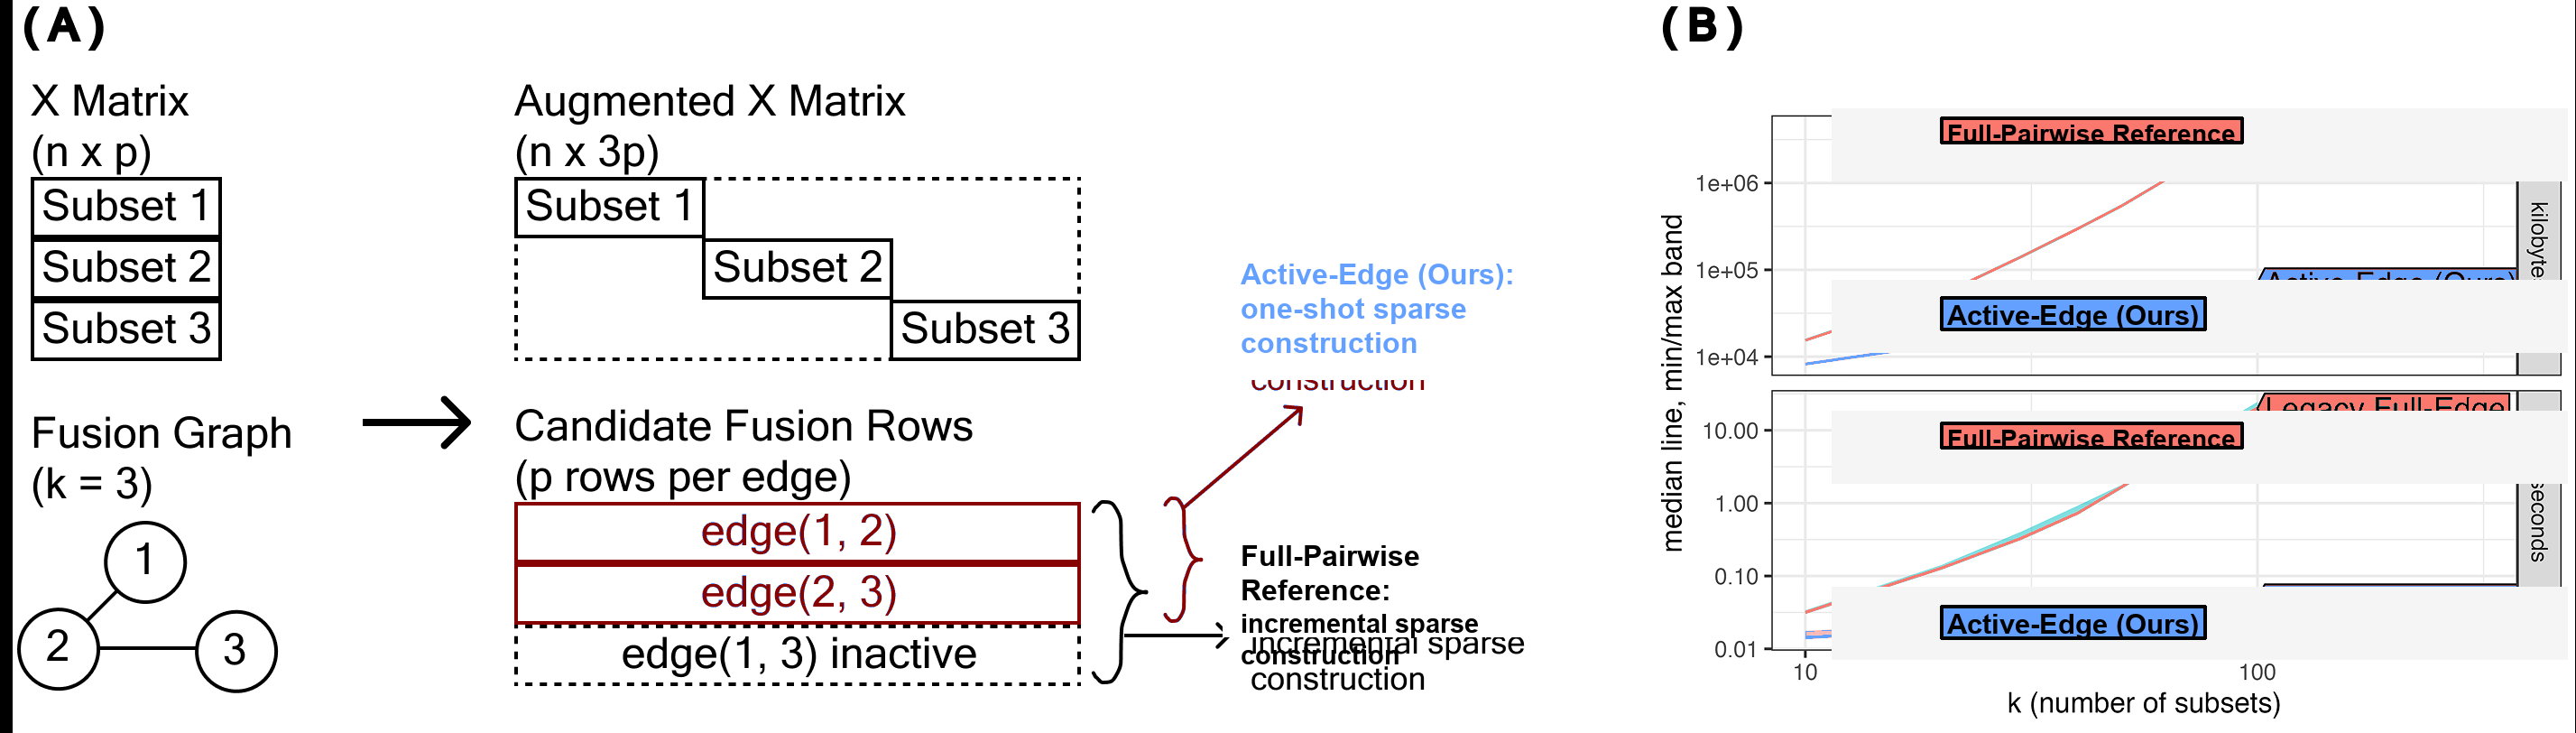
\includegraphics[width=1\textwidth]{figures/concept2.png}
  \caption{Conceptual overview of L2 sparse-graph fusion. 
  A: augmented matrix construction. 
  The reference full-edge construction associated with \citet{dondelinger2020joint} forms augmented rows for all group pairs, while the active-edge builder emits only sparse triplets for graph edges with nonzero weight. 
  B: asymptotic complexity. 
  The synthetic example uses $p=120$ features and 35 training observations per group, so when $k=100$ the training set has $n=3500$ observations. 
  For the sparse chain graph, where $m$ is the number of fusion edges ($m=k-1$), active-edge construction changes the dominant fusion-block cost from $O(pk^2)$ to $O(pm)$.
  }
  \label{fig:concept-l2}
\end{figure}


\subsection{Optimization Guarantee for Smoothed L1}
The L1 solver follows a smoothed proximal-gradient strategy for Equation~\ref{eq:model}. 
Let $B=[\beta_1,\ldots,\beta_k]$ be the $p \times k$ coefficient matrix. 
The reference implementation builds a constraint matrix with columns for sparsity and fusion constraints, then uses a smoothed dual approximation to compute the gradient contribution of the nonsmooth penalty.
The update has the generic accelerated form
\begin{align}
  A^\star &= \Pi_{[-1,1]}\left(\frac{B C}{\mu}\right),\\
  \nabla f_\mu(B) &= \nabla \ell(B) + A^\star C^\top,\\
  B^{t+1} &= W^t - L^{-1}\nabla f_\mu(B^t),
\end{align}
where $C$ encodes the sparsity and fusion operators, $\mu$ is the smoothing parameter, $L$ is a Lipschitz bound, and $W^t$ is the accelerated iterate.
When $C$ contains all group pairs, storage and multiplication include $O(pk^2)$ fusion terms for a complete representation.
More explicitly, the L1 implementation uses the dual identity $|z|=\max_{|a|\leq 1} az$ and replaces the non-smooth absolute value terms by clipped smoothed duals. 
For sparsity and active fusion edges this gives
\[
  A_s^\star = \clip\left(\frac{\lambda B_s}{\mu}, -1, 1\right),
  \qquad
  A_{uv}^\star =
  \clip\left(\frac{\gamma w_{uv}(\beta_u-\beta_v)}{\mu}, -1, 1\right),
\]
where $B_s$ excludes intercept rows. The code uses the step-size upper bound
\[
  L_U =
  \lambda_{\max}
  + \frac{\lambda^2+2\gamma^2 d_{\max}^{(2)}}{\mu},
\]
with $\lambda_{\max}=\sum_g \lambda_{\max}(X_g^\top X_g/n_g)$ under scaled group losses and $d_{\max}^{(2)}$ any upper bound on
$\max_g\sum_{h:(g,h)\in E} w_{gh}^2$ for the active fusion graph. 
This quantity is bounded by the usual weighted degree when weights are normalized to lie in $[0,1]$.
The guarantees below are deterministic statements for a fixed graph and fixed hyper-parameters. 
They concern objective representation and optimization, not statistical recovery under a data generating model.
The first guarantee specializes the standard consequences of Nesterov smoothing and accelerated proximal-gradient convergence to the grouped fused-regression notation used here \citep{nesterov2005smooth,beck2009fast}.

\begin{proposition}[Lipschitz and convergence guarantee for smoothed L1]
\label{prop:l1-convergence}
\leavevmode\par\noindent
Let $F_\mu(B)$ be the Nesterov-smoothed L1 grouped fused objective, before final postprocessing. 
Let $B_\mu^\star$ minimize $F_\mu$. 
If the Accelerated Proximal Gradient (APG) update uses any $L_U$ satisfying
\[
  L_U \geq
  \lambda_{\max}
  + \frac{\lambda^2+2\gamma^2 d_{\max}^{(2)}}{\mu},
\]
then $\nabla F_\mu$ is $L_U$-Lipschitz and the accelerated iterates satisfy
\[
  F_\mu(B^{(t)})-F_\mu(B_\mu^\star)
  \leq
  \frac{2L_U\norm{B^{(0)}-B_\mu^\star}_F^2}{(t+1)^2}.
\]
Moreover, if $N_c$ is the number of scalar sparsity and fusion constraints in the active-edge representation, then the nonsmoothed objective $F$ and its smoothed version obey
\[
  0 \leq F(B)-F_\mu(B) \leq \frac{\mu N_c}{2}
\]
for every coefficient matrix $B$.
\end{proposition}

\begin{proof}
The least-squares part has Lipschitz constant bounded by $\lambda_{\max}$ under the scaled group losses. 
The smoothed sparsity operator contributes at most $\lambda^2/\mu$ to the gradient Lipschitz constant. 
For the fusion operator, each edge difference has two incident group blocks. 
The squared operator norm is bounded by $2d_{\max}^{(2)}$, giving the fusion contribution $2\gamma^2 d_{\max}^{(2)}/\mu$. 
Summing these bounds gives $L_U$. 
The stated $O(t^{-2})$ rate is the standard accelerated-gradient guarantee for convex differentiable objectives with $L_U$-Lipschitz gradient. 
Finally, each scalar absolute-value term satisfies $0\leq |z|-\max_{|a|\leq 1}\{az-\mu a^2/2\}\leq\mu/2$; summing over the $N_c$ scalar constraints gives the smoothing gap.
\end{proof}

\begin{proposition}[Equivalence of dense and active-edge L1 gradients]
\label{prop:l1-equivalence}
\leavevmode\par\noindent
Fix a weighted graph $G$ and let $E$ denote the edges with positive weight.
For smoothing parameter $\mu>0$, suppose the dense smoothed proximal-gradient implementation includes one fusion column for every pair but assigns zero weight to inactive pairs. 
The active-edge operator implementation computes exactly the same smoothed fusion gradient as the dense implementation after removing the zero-weight columns.
\end{proposition}

\begin{proof}
Let $e_u$ be the $u$th coordinate vector in $\R^k$. For any pair
$1\leq u<v\leq k$, define the smoothed dual block
\[
  P_{uv}(B)
  =
  \clip\left(
  \frac{\gamma w_{uv}(\beta_u-\beta_v)}{\mu},-1,1
  \right).
\]
The dense fusion contribution to the smoothed gradient can be written as
\[
  \Delta_{\mathrm{dense}}(B)
  =
  \sum_{1\leq u<v\leq k}
  \gamma w_{uv} P_{uv}(B)(e_u-e_v)^\top .
\]
If $w_{uv}=0$, then the corresponding summand is zero. Therefore
\[
  \Delta_{\mathrm{dense}}(B)
  =
  \sum_{(u,v)\in E}
  \gamma w_{uv} P_{uv}(B)(e_u-e_v)^\top
  =
  \Delta_{\mathrm{active}}(B).
\]
Algorithm~\ref{alg:active_edge_operator} computes this last expression by adding $\gamma w_{uv}P_{uv}(B)$ to column $u$ and subtracting it from column $v$ for each active edge. 
Hence the dense and active-edge implementations produce the same smoothed fusion-gradient contribution, and therefore the same L1 update when the remaining APG quantities are held fixed.
\end{proof}

\begin{algorithm}[H]
\caption{Full-Pairwise APG Reference}
\label{alg:old_l1}
\begin{algorithmic}[1]
\Require grouped data, $G$, $\lambda,\gamma,\mu,T,\varepsilon$
\State Construct full fusion matrix $C_{\mathrm{fusion}}\in\R^{k\times \binom{k}{2}}$
\State Construct $C=[\lambda I_k,\gamma C_{\mathrm{fusion}}]$
\State Initialize $B^{(0)}=0,\;W^{(0)}=0,\;S^{(0)}=0$
\For{$t=1,\dots,T$}
  \State Compute $\nabla \ell(B^{(t-1)})$ groupwise
  \State $A^\star\gets
  \clip\!\left([B_s^{(t-1)}C_s,\;B_f^{(t-1)}C_f]/\mu,-1,1\right)$
  \State $\nabla r_\mu(B^{(t-1)})\gets A^\star C^\top$
  \State $H_t \gets \nabla \ell(B^{(t-1)})+\nabla r_\mu(B^{(t-1)})$
  \State Compute $L_U$ from the dense max-degree proxy
  \State Update $\tilde B^{(t)},S^{(t)},W^{(t)}$
  \If{$\norm{\tilde B^{(t)}-B^{(t-1)}}_1<\varepsilon p$}
    \State \textbf{break}
  \EndIf
  \State $B^{(t)}\gets \tilde B^{(t)}$
\EndFor
\State Soft-threshold non-intercept rows by $\lambda/n_g$
\State \Return $\hat B$
\end{algorithmic}
\end{algorithm}


\subsection{Full-Edge L2 Augmented Design}
The L2 solver uses a different reduction. 
It constructs an augmented response and design matrix,
\[
  \tilde y =
  \begin{bmatrix} y \\ 0 \end{bmatrix}, \quad
  \tilde X =
  \begin{bmatrix} X_{\mathrm{block}} \\ X_{\mathrm{fusion}} \end{bmatrix},
\]
where $X_{\mathrm{block}}$ is block diagonal over groups and $X_{\mathrm{fusion}}$ contains, for each group pair, rows proportional to
\[
  \sqrt{\gamma w_{gh}}(\beta_g-\beta_h).
\]
The resulting lasso problem is passed to \texttt{glmnet}. 
A full all-pairs construction creates $O(p k^2)$ fusion rows even when only $m=|E|$ edges are active.

\begin{proposition}[Equivalence of active-edge L2 augmented rows]
\label{prop:l2-equivalence}
For a fixed graph $G$, penalty $\gamma$, and scaling convention, the active-edge L2 augmented design is equivalent to the all-pairs augmented design after removing all zero-weight pair rows and applying a row permutation.
The active-edge L2 design gives the same optimization problem as the all-pairs design, except it omits rows that were zero anyway.
\end{proposition}

\begin{proof}
Each nonzero edge $(u,v)$ contributes $p_{\mathrm{eff}}$ augmented rows with $+\sqrt{\gamma w_{uv}}$ in coefficient block $u$ and $-\sqrt{\gamma w_{uv}}$ in coefficient block $v$, with zero augmented response. 
These rows contribute
\[
  \gamma w_{uv}\norm{\beta_u-\beta_v}_2^2
\]
to the augmented least-squares objective. 
Therefore the all-pairs fusion contribution satisfies
\[
  \sum_{1\leq u<v\leq k}
  \gamma w_{uv}\norm{\beta_u-\beta_v}_2^2
  =
  \sum_{(u,v)\in E}
  \gamma w_{uv}\norm{\beta_u-\beta_v}_2^2,
\]
because inactive pairs have $w_{uv}=0$. 
The active-edge builder constructs exactly the rows corresponding to the right-hand side using sparse triplets.
Permuting those rows changes only their order, not the sum of squared residuals, so the objective minimized by \texttt{glmnet} is unchanged.
\end{proof}

\begin{proposition}[Sparse-graph construction cost]
\label{prop:complexity}
\leavevmode\par\noindent
Let $k$ be the number of groups, $p$ the number of penalized coefficients per group, $m=|E|$ the number of nonzero fusion edges, and $q=\binom{k}{2}$ the number of all possible group pairs. 
In one L1 smoothed-gradient evaluation, a dense all-pairs operator performs fusion work proportional to $pq$ after construction, whereas the active-edge operator performs fusion work proportional to $pm$. 
In the L2 augmented-design construction, the fusion block decreases from $pq$ augmented rows to $pm$
augmented rows.
\end{proposition}

\begin{proof}
For L1 fusion, each represented edge requires a $p$-dimensional coefficient difference and a $p$-dimensional scatter back to the incident groups. 
Thus, the fusion-side work scales as
\[
  W_{\mathrm{L1,full}} \asymp p q
  =
  p\binom{k}{2},
  \qquad
  W_{\mathrm{L1,active}} \asymp p m .
\]
The dense all-pairs representation iterates over $q$ candidate pairs, including zero-weight inactive pairs, while the active-edge representation iterates only over the $m$ nonzero graph edges.

For L2 fusion, each represented edge contributes $p_{\mathrm{eff}}$ augmented rows, one for each penalized coefficient coordinate. 
Therefore the fusion block sizes are
\[
  R_{\mathrm{L2,full}} = p_{\mathrm{eff}} q
  =
  p_{\mathrm{eff}}\binom{k}{2},
  \qquad
  R_{\mathrm{L2,active}} = p_{\mathrm{eff}} m .
\]
Deleting zero-weight pairs gives the stated row reduction, with $p_{\mathrm{eff}}$ determined by the intercept convention.
\end{proof}

\section{Sparse-Graph Solvers}
\label{sec:solvers}

\subsection{Exact L1 Operator Solver}
Here $B=[\beta_1,\ldots,\beta_k]$ is the grouped coefficient matrix, with one column per group. 
The exact L1 operator solver replaces the dense fusion matrix representation with edge lists $(u_e,v_e,w_e)_{e=1}^m$, where $m=|E|$ is the number of active fusion edges, $u_e$ and $v_e$ are the incident groups for edge $e$, and $w_e>0$ is its fusion weight. 
At each iteration, the solver computes the fusion differences only on active edges,
\[
  D_e = \beta_{u_e}-\beta_{v_e},
  \quad
  P_e = \clip\left(\frac{\gamma w_e D_e}{\mu},-1,1\right),
\]
where $D_e$ is the coefficient difference vector and $P_e$ is its clipped smoothed dual block. 
The solver scatters $\gamma w_e P_e$ back to the incident group columns with opposite signs. 
The sparsity part of the update remains unchanged. 
This representation has the same objective and first-order updates as the active-edge version of the smoothed proximal-gradient solver, but the fusion-gradient work scales with $pm$ rather than $pk^2$.

The implementation also supports block processing of edges. 
This is a practical memory safeguard for large $p$ or $m$, since intermediate edge-difference matrices can otherwise dominate the working set.
The operator solver is therefore intended as the general exact path for sparse graphs.

\paragraph{Active-edge gradient assembly.}
The implementation forms the fusion-gradient contribution by initializing $\Delta_f=0$ and looping over active edges $e=1,\ldots,m$. 
For each edge, it computes the per-edge difference $d_e=\beta_{u_e}-\beta_{v_e}$ and clipped dual block $p_e=\clip((\gamma w_e/\mu)d_e,-1,1)$, then applies the scatter updates
\[
  \Delta_f(:,u_e) \leftarrow \Delta_f(:,u_e)+\gamma w_e p_e,
  \qquad
  \Delta_f(:,v_e) \leftarrow \Delta_f(:,v_e)-\gamma w_e p_e.
\]
The accumulated matrix $\Delta_f$ is then added to the likelihood and sparsity gradient terms in the accelerated update.

\paragraph{Algorithm.}
Algorithm~\ref{alg:active_edge_operator} gives the active-edge APG procedure used in the experiments. 
Here, $T$ is the maximum number of APG iterations and $\varepsilon$ is the stopping tolerance.

\begin{algorithm}[H]
\caption{Active-Edge Operator APG}
\label{alg:active_edge_operator}
\begin{algorithmic}[1]
\Require grouped data, edge list $E$, $\lambda,\gamma,\mu,T,\varepsilon$
\State Initialize $B^{(0)}=0,\;W^{(0)}=0,\;S^{(0)}=0$
\For{$t=1,\dots,T$}
  \State Compute groupwise likelihood gradient $\nabla \ell(B^{(t-1)})$
  \State $A_s^\star \gets \clip(\lambda B_s^{(t-1)}/\mu,-1,1)$
  \State Initialize fusion accumulator $\Delta_f \gets 0$
  \For{each edge $e=(u_e,v_e,w_e)\in E$}
     \State $d_e \gets \beta_{u_e}^{(t-1)}-\beta_{v_e}^{(t-1)}$
     \State $p_e \gets \clip((\gamma w_e/\mu)d_e,-1,1)$
     \State $\Delta_f(:,u_e) \gets \Delta_f(:,u_e)+\gamma w_e p_e$
     \State $\Delta_f(:,v_e) \gets \Delta_f(:,v_e)-\gamma w_e p_e$
  \EndFor
  \State $H_t \gets \nabla \ell(B^{(t-1)}) + \lambda A_s^\star + \Delta_f$
  \State Compute $L_U$ on active graph; update $\tilde B^{(t)},S^{(t)},W^{(t)}$
  \If{$\norm{\tilde B^{(t)}-B^{(t-1)}}_1 < \varepsilon p$}
    \State \textbf{break}
  \EndIf
  \State $B^{(t)}\gets \tilde B^{(t)}$
\EndFor
\State Soft-threshold non-intercept rows by $\lambda/n_g$
\State \Return $\hat B$
\end{algorithmic}
\end{algorithm}

\subsection{Chain Approximation}

The chain approximation solver builds a depth-first traversal of a maximum spanning tree or of the thresholded graph, reorders the groups along that traversal, and keeps only the $k-1$ adjacent chain edges.
The fusion operator can then be computed with vectorized adjacent differences:
\[
  D_j = \beta_j-\beta_{j+1}, \quad j=1,\ldots,k-1.
\]
The vectorized implementation forms
\[
  D = B_{:,1:(k-1)} - B_{:,2:k}, \qquad
  P = \clip((\gamma/\mu)D\operatorname{diag}(w),-1,1),
\]
and accumulates $\gamma P\operatorname{diag}(w)$ on neighboring chain endpoints.
This reduces the edge budget to the minimum needed to connect the groups. 
It does not optimize the same objective as the original graph unless the graph is already the selected chain. 
It is useful when the main objective is maximum speed and memory reduction and the user is willing to accept a small loss in graph fidelity.

\begin{proposition}[Chain approximation target]
\label{prop:chain-target}
\leavevmode\par\noindent
Let $G_\pi=(V,E_\pi)$ be the chain graph produced by the DFS/MST ordering, with edge weights inherited from the original graph. 
The chain approximation solver applies the exact active-edge L1 update to the smoothed fused objective on $G_\pi$. 
Define the original graph-fusion penalty as
\[
  R_G(B)=\gamma\sum_{(u,v)\in E}
  w_{uv}\norm{\beta_u-\beta_v}_1,
\]
and define $R_{G_\pi}(B)$ analogously on the chain. 
Then, for any coefficient matrix $B$ and any chain with $E_\pi\subseteq E$,
\[
  0 \leq R_G(B)-R_{G_\pi}(B)
  =
  \gamma\sum_{(u,v)\in E\setminus E_\pi}
  w_{uv}\norm{\beta_u-\beta_v}_1.
\]
Thus, the approximation error is exactly the omitted-edge fusion penalty for the fitted coefficient matrix.
\end{proposition}

\begin{proof}
After the groups are reordered by $\pi$, the vectorized adjacent-difference operator is the active-edge operator for the chain edges $(\pi_j,\pi_{j+1})$, $j=1,\ldots,k-1$. 
The scatter updates therefore match the L1 active-edge update on $G_\pi$. 
Moreover,
\[
  R_G(B)-R_{G_\pi}(B)
  =
  \gamma\sum_{(u,v)\in E}w_{uv}\norm{\beta_u-\beta_v}_1
  -
  \gamma\sum_{(u,v)\in E_\pi}w_{uv}\norm{\beta_u-\beta_v}_1.
\]
If $E_\pi\subseteq E$, the second sum removes exactly the retained chain edges, leaving
\[
  R_G(B)-R_{G_\pi}(B)
  =
  \gamma\sum_{(u,v)\in E\setminus E_\pi}
  w_{uv}\norm{\beta_u-\beta_v}_1
  \geq 0.
\]
\end{proof}

\paragraph{Optimization algorithm.}
The chain approximation algorithm first builds the DFS/MST order and adjacent chain weights, then runs a separate vectorized APG routine rather than calling the general edge loop. 
In Algorithm~\ref{alg:chain_approx}, $\eta=1/L_U$ is the step size, $H_t$ is the smoothed gradient at iteration $t$, $R^{(t)}$ is the accumulated scaled-gradient term, $Z^{(t)}=-R^{(t)}$ is the aggregate point used in the acceleration step, and $W^{(t)}$ is the accelerated iterate:
\begin{algorithm}[H]
\caption{Chain Approximation APG}
\label{alg:chain_approx}
\begin{algorithmic}[1]
\Require grouped data, $G$, chain settings, $\lambda,\gamma,\mu,T,\varepsilon$
\State Build DFS/MST chain order $\pi$ and adjacent chain weights $(w_1,\dots,w_{k-1})$
\State Reorder groups by $\pi$; initialize $B^{(0)}=0,\;W^{(0)}=0,\;R^{(0)}=0$
\State Compute chain Lipschitz bound $L_U$ and set $\eta\gets 1/L_U$
\For{$t=1,\dots,T$}
  \State Compute groupwise likelihood gradient $\nabla \ell(B^{(t-1)})$
  \State $A_s^\star\gets\clip(\lambda B_s^{(t-1)}/\mu,-1,1)$
  \State $\Delta_f(:,1:(k-1)) \mathrel{+}= C,\qquad
  \Delta_f(:,2:k) \mathrel{-}= C$
  \State $H_t\gets \nabla \ell(B^{(t-1)})+\lambda A_s^\star+\Delta_f$
  \State $\tilde B^{(t)}\gets W^{(t-1)}-\eta H_t$
  \State $R^{(t)}\gets R^{(t-1)}+\frac{t\eta}{2}H_t$
  \State $Z^{(t)}\gets -R^{(t)}$
  \State $W^{(t)}\gets \left(t\tilde B^{(t)}+2Z^{(t)}\right)/(t+2)$
  \If{$\norm{\tilde B^{(t)}-B^{(t-1)}}_1<\varepsilon p$}
    \State \textbf{break}
  \EndIf
  \State $B^{(t)}\gets \tilde B^{(t)}$
\EndFor
\State Soft-threshold non-intercept rows by $\lambda/n_g$
\State Reorder columns back to original group order
\State \Return $\hat B$
\end{algorithmic}
\end{algorithm}



\subsection{Active-Edge L2 Augmented Design}

The L2 active-edge solver preserves the augmented-design strategy but changes how the design is built.  
Instead of allocating all pairwise fusion blocks and then assigning zero-weight rows, it finds the upper-triangular nonzero entries of $G$ and builds sparse triplets only for those edges. 
The $p_{\mathrm{eff}}$ denotes the number of coefficient coordinates included in the L2 fusion block, and $n_{\mathrm{fusion}}=p_{\mathrm{eff}}m$ is the number of active fusion rows. 

The active-edge construction keeps the same augmented-design scaling:
\[
  \sqrt{\gamma(n+n_{\mathrm{fusion}})}\sqrt{w_{gh}}
\]
multiplies the positive and negative entries in the fusion rows. 
The final augmented design is passed to \texttt{glmnet} \citep{glmnet} with the lambda correction factor.
This change leaves the fitted objective unchanged for a given active graph but reduces the number of constructed fusion rows from $p_{\mathrm{eff}} k(k-1)/2$ to $p_{\mathrm{eff}}m$. 
The largest expected gains occur when $m \ll k(k-1)/2$.

\paragraph{Optimization algorithm.}
The L2 path uses \texttt{glmnet} \citep{glmnet} after building an augmented sparse regression problem. 
The fitted vector $\theta$ stacks the groupwise coefficients and is reshaped into the coefficient matrix $B$ after fitting:
\begin{algorithm}[t]
\caption{L2 Augmented Design Solver with \texttt{glmnet}}
\label{alg:l2_augmented_design}
\begin{algorithmic}[1]
\Require grouped data $(X,y,\mathrm{groups})$, graph $G$, $\lambda,\gamma$, intercept and loss-scaling conventions
\State Build block-diagonal design $X_{\mathrm{block}}$ over groups
\State Extract active edges $E=\{(u,v):u<v,\;G_{uv}\ne 0\}$
\State Let $\mathcal P$ be the coefficient coordinates included in L2 fusion, with $|\mathcal P|=p_{\mathrm{eff}}$
\State Initialize sparse triplet lists for $X_{\mathrm{fusion}}$ and set row counter $a\gets 0$
\For{each active edge $(u,v)\in E$}
  \For{each coefficient coordinate $r\in\mathcal P$}
    \State $a\gets a+1$
    \State Add triplet $(a,\operatorname{col}(u,r),+\sqrt{w_{uv}})$
    \State Add triplet $(a,\operatorname{col}(v,r),-\sqrt{w_{uv}})$
  \EndFor
\EndFor
\State Set $n_{\mathrm{fusion}}\gets a$ and materialize sparse matrix
$X_{\mathrm{fusion}}$ from the triplets
\State Scale fusion block by $\sqrt{\gamma(n+n_{\mathrm{fusion}})}$
\State Form augmented system $\tilde X=[X_{\mathrm{block}};X_{\mathrm{fusion}}]$, $\tilde y=[y;0]$
\State Fit $\theta$ with \texttt{glmnet} on $(\tilde X,\tilde y)$ using $\lambda$
\State Reshape $\theta$ to $B\in\R^{p_{\mathrm{eff}}\times k}$
\State \Return $B$
\end{algorithmic}
\end{algorithm}

Table~\ref{tab:complexity} summarizes the asymptotic costs implied by the preceding solver descriptions. 
The purpose is to separate the common groupwise regression cost, represented by $O(np)$ terms, from the cost of the fusion representation. 
The L1 time entries describe one APG iteration, while the L2 time entries describe one pass over the augmented design. 
For L2, the table uses $p_{\mathrm{eff}}$ because the intercept convention determines how many coefficient coordinates are included in the fusion block. 
The active-edge L1 memory bound assumes the block processing, so edge-difference workspaces are not materialized for all $m$ edges at once.

\begin{table}[t]
\centering
\caption{Dominant representation costs of the solver methods.
Here $n$ is total sample size, $p$ is feature count, $p_{\mathrm{eff}}$ is the number of coordinates included in the L2 fusion block, $k$ is group count,
$m=|E|$ is the number of active fusion edges, and $q=\binom{k}{2}$. 
The table isolates graph-representation costs and omits lower-order constants from solver overhead.}
\label{tab:complexity}
\begin{tabular}{lll}
\toprule
Method & Time & Memory \\
\midrule
L1 Full-Pairwise Reference & $O(np+pkq)$ & $O(np+pk+pq+kq)$ \\
L1 Active-Edge & $O(np+pm)$ & $O(np+pk+m)$ \\
L1 Chain Approximation & $O(np+pk)$ & $O(np+pk)$ \\
\midrule
L2 Full-Pairwise Reference & $O(np+p_{\mathrm{eff}}q)$ & $O(np+p_{\mathrm{eff}}q)$ \\
L2 Active-Edge & $O(np+p_{\mathrm{eff}}m)$ & $O(np+p_{\mathrm{eff}}m)$ \\
\bottomrule
\end{tabular}
\end{table}


\section{Experimental Design}

\subsection{Empirical Test Problems}

The real data experiments use public grouped regression problems as optimization test cases. 
They provide different values of $n$, $p$, $k$, and graph sparsity while keeping the statistical objective fixed across solver representations. 
Across these datasets, the number of observations ranges from 630 to 200,000, the number of features from 3 to 100, and the number of groups from 43 to 229. 
Most of the real data test problems are drawn from Rdatasets mirrors \citep{rdatasets}. 
The remaining sources are UCI datasets \citep{uci_communities,uci_electricity}, Our World in Data CO2 data \citep{owidco2}, World Bank indicators \citep{worldbankwdi}, and package datasets \citep{pinheiro2000mixed,raudenbush2002hlm}. 

\subsection{Evaluation Protocol}
All reported real data results use grouped outer cross-validation with five stratified folds \citep{kohavi1995cross,varma2006bias}. 
Splits are made at the observation level while preserving group representation where possible.
All graph construction, hyperparameter selection, and standardization are performed inside the outer-training fold so that the held-out test fold is not used in model selection.

For each outer fold, a baseline sparsity penalty is selected with fusion disabled, $\gamma=0$, on the outer-training data by \texttt{cv.glmnet} with three inner folds and \texttt{lambda.min}. 
We denote this selected sparsity penalty by $\lambda$ in Equation~\ref{eq:model}. 
Holding this $\lambda$ fixed, a separate inner train-validation split of the outer-training data selects the fusion penalty $\gamma$ in Equation~\ref{eq:model} by validation root mean squared error (RMSE).
The goal of the experiments is to compare solver representations under a common protocol, not to optimize hyperparameter-search efficiency.
It was sufficient to select nontrivial fused models that outperform the featureless baseline in the reported result panels. 
The final model is then refit on the full outer-training fold using the selected $\lambda$ and $\gamma$ and evaluated on the held-out outer fold. 
The featureless baseline predicts the mean of the training fold for the corresponding response. 
Timing measures only the model-fitting step, and memory is the maximum RAM used by the fitting process.

The experiments were run on Northern Arizona University's Monsoon cluster, an
x86\_64 Linux cluster running Red Hat Enterprise Linux 8 and scheduled with
Slurm \citep{nau_monsoon}. 
The package was evaluated in R, with R and Rcpp/C++ code linked against the
BLAS and LAPACK libraries available through R. 
Timing experiments were submitted as Slurm array jobs with one CPU core per
task and a 24-hour time limit. 
Jobs were split into small, medium, and large memory tiers and requested 16 GB,
32 GB, and 64 GB of memory, respectively. 
The tier assignment used a deterministic workload score based on $n$, $p$, and
$k$ of the data.
The job scripts do not request exclusive allocation or pin jobs to a particular
Monsoon node generation, so absolute wall-clock times may reflect normal
shared-cluster and hardware variability. 
For this reason, timing results are interpreted primarily as relative
comparisons between solver representations run under the same scheduling
protocol.


\subsection{Graph Construction and Hyperparameters}
The real data benchmark constructs a data-driven group graph from training data, following the use of graph-based relationships and k-nearest-neighbor fusion graphs in prior work \citep{hallac2015network,padilla2020adaptive}.
Group centroids are computed on the outer-training fold, a k-nearest-neighbor graph is formed from centroid distances, inverse-distance weights are used, and connectivity is enforced by adding nearest inter-component links.
Graphs are constructed using \(k=5\) nearest neighbors \citep{hallac2015network,padilla2020knn}, inverse-distance edge weights \citep{hallac2015network}, and minimum-spanning-tree augmentation to ensure connectivity.

This follows the general idea that graph structure should encode similarity between groups rather than defaulting to a complete graph.
A complete graph may still be appropriate when every group pair is intended to be fused, but in that case the active-edge representation has $m=\binom{k}{2}$ and therefore does not provide the sparse-graph efficiency gains targeted in this paper.
Each dataset is evaluated with five outer folds. 
The regularization parameter $\lambda$ is warm-started from \texttt{cv.glmnet}; the fusion parameter $\gamma$ is selected from the grid $10^{-6}$ to $10^{-1}$.
The L1 optimization tolerance is $10^{-5}$ with a maximum of 1200 iterations.
% Runs use intercepts for L1 models, no feature scaling inside the L1 solver, standardized inputs for benchmark construction, an edge-block size of 256 for the operator implementation. 
The L2 panel uses the same outer-fold and graph protocol with the L2 solvers.

\subsection{Compared Methods}
For L1 fusion, we compare the reference full construction, the exact active-edge operator, the chain approximation, and a featureless baseline. 
For L2 fusion, we compare the reference augmented design, the active-edge augmented design, and the featureless baseline.

The exact comparisons are intentionally conservative. 
The operator and active-edge L2 methods are compared against reference implementations using the same graph, outer folds, selected hyperparameters, and prediction pipeline.
Thus the reported differences isolate representation and construction costs, not changes in the statistical model or optimizer family.
Comparisons against ADMM \citep{boyd2011admm,hallac2015network}, split-Bregman \citep{ye2011split}, or other edge-splitting optimizers answer a broader question about optimizer choice.
The present experiments instead test whether the sparse graph can be preserved while keeping the L1 solver within the smoothed proximal-gradient family \citep{chen2012smoothing} and the L2 solver within the augmented-design family.
The chain-approximation L1 method is reported separately because it changes the graph and is therefore an approximation rather than an exact replacement.

\section{Results}

The first experiment illustrates when graph fusion is statistically useful relative to unfused \texttt{glmnet} baselines. 
The remaining results evaluate the main optimization question of the paper, namely whether sparse-graph representations preserve predictive accuracy while reducing runtime and memory for L1 and L2 grouped fused regression.


\begin{figure}[t]
  \centering
  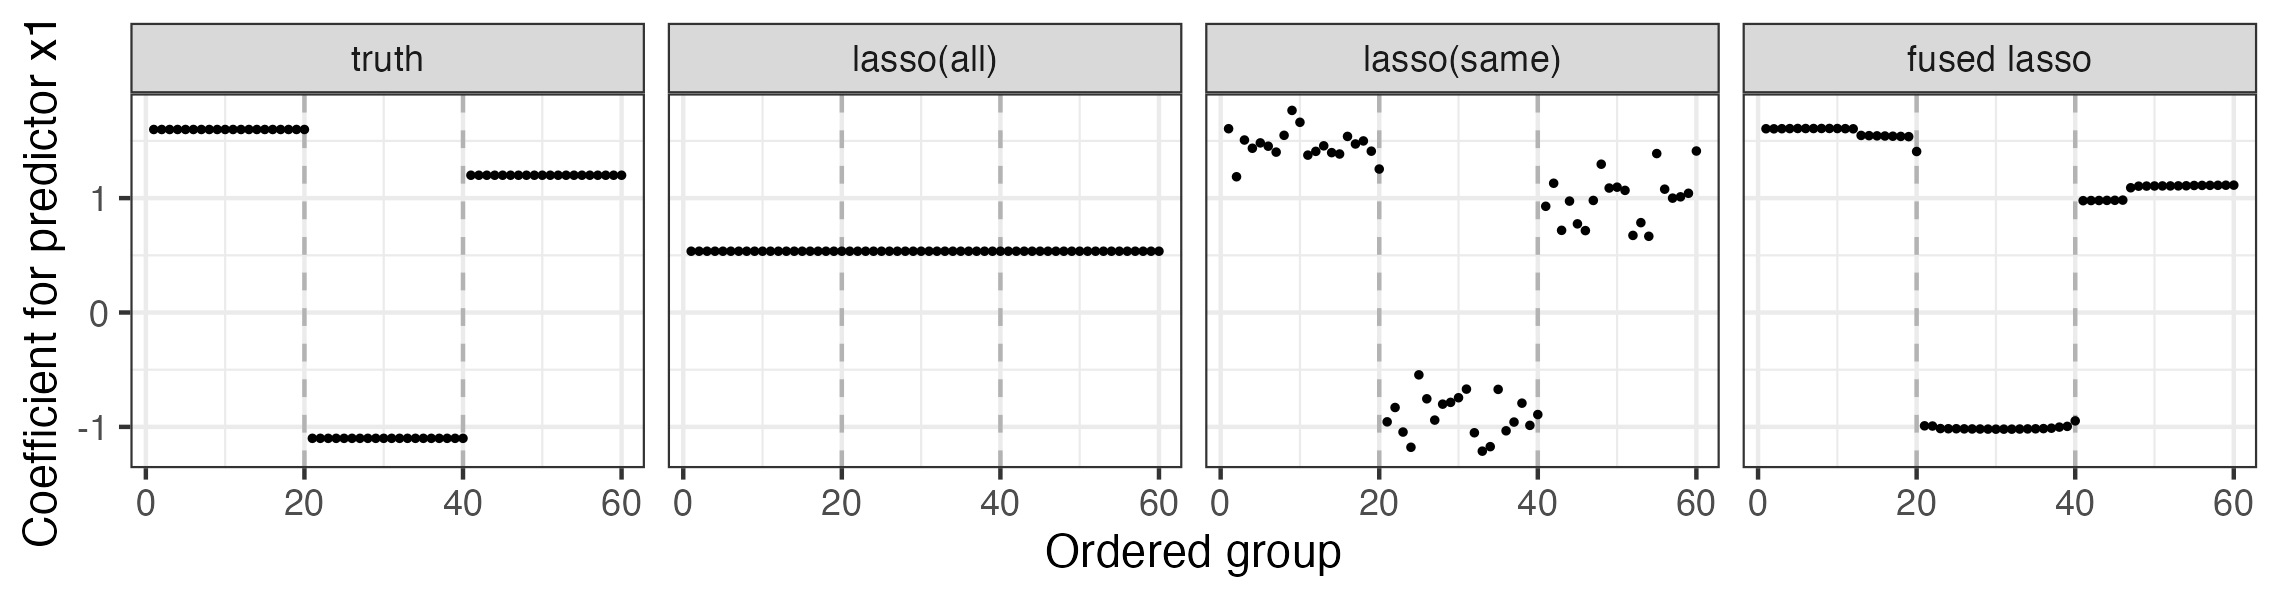
\includegraphics[width=1\textwidth]{figures/changepoint_fused_vs_glmnet.png}
  \caption{Controlled changepoint example comparing fused regression with unfused lasso baselines. 
  Points show the coefficient for the first predictor across all 60 ordered groups, and dashed vertical lines mark the true changepoints. 
  lasso(all) fits only one shared coefficient path, lasso(same) produces noisy separate paths, and the fused lasso model recovers the piecewise-constant coefficient structure.
  The lasso baselines are fit with \texttt{glmnet}.}
  \label{fig:changepoint-glmnet}
\end{figure}


\subsection{Changepoint Structure and the Need for Fusion}
Before comparing solver representations, we first show a case where fusion is statistically useful relative to unfused lasso baselines. 
Unfused lasso regression implementations such as \texttt{glmnet} are highly optimized and computationally efficient. 
When the application does not require fusion across groups, these baselines are certainly preferable to fused-regression alternatives.
The purpose of this experiment is to clarify why a fused lasso regression model is even useful in the first place.
The data generation process has ordered groups whose regression coefficients are neither globally identical nor unrelated across groups.
The intended structure is piecewise constant across three contiguous blocks: groups 1--20, groups 21--40, and groups 41--60 each have stable coefficients, with changes only at the two boundaries between these blocks.
We generated an ordered-group regression problem with $k=60$ groups and $p=20$ predictors. 
The true coefficient paths are piecewise constant: groups 1--20 share one coefficient block, groups 21--40 share a second block, and groups 41--60 share a third block. 
Therefore, the two true changepoints occur after groups 20 and 40. 
Each group has 25 training observations for fitting, 10 validation observations for tuning, and 80 test observations. 
The fusion graph is the chain over the ordered groups, so the fused model penalizes differences only between neighboring groups.

We compare three estimators. 
The lasso(all) baseline fits one shared coefficient vector using all groups together, so it is stable but cannot represent changepoints for each group.
The lasso(same) baseline uses interaction terms to fit separate coefficient vectors for each group without any fusion penalty. 
It does not borrow strength across neighboring groups.
The fused lasso model also estimates coefficient vectors for each group, but adds an L1 fusion penalty on adjacent groups in the chain so that it balances shared signal against differences among groups.
Both lasso baselines are fit with \texttt{glmnet}.
Their lasso penalties are selected by five-fold \texttt{cv.glmnet} on the training data, while the fused lasso selects $(\lambda,\gamma)$ by validation RMSE over a fixed grid.

Figure~\ref{fig:changepoint-glmnet} shows the fitted path for the first predictor across the 60 ordered groups. 
The lasso(all) path is nearly flat because it must use the same coefficient vector for all groups. 
The lasso(same) path varies by group, but without fusion it produces a noisy path with many spurious jumps. 
The fused lasso path is piecewise constant and changes at the two true changepoints. 

Numerically, the fused lasso obtains the lowest test RMSE (0.708), the lowest relative coefficient error (0.079), and exactly two large estimated jumps, both at the true changepoints. 
By comparison, lasso(all) has test RMSE 1.957 and relative coefficient error 0.848, while lasso(same) improves prediction error but produces 59 large jumps.

\begin{figure}[t]
  \centering
  
\includegraphics[width=\textwidth]{figures/hpc_l1_l2_three_datasets.png}
  \caption{Prediction accuracy for L1 and L2 fusion on real grouped regression datasets. 
  Points show test RMSE means over five cross-validation folds, with horizontal bars showing the standard deviation. 
  The vertical red lines indicate the full pairwise baseline error which we want to preserve with the other methods.
  Exact active-edge solvers preserve the full-construction RMSE, while the chain approximation is an approximate method.}
  \label{fig:l1-l2-accuracy-three-datasets}
\end{figure}

\subsection{Accuracy Preservation}
Figure~\ref{fig:l1-l2-accuracy-three-datasets} compares prediction accuracy for L1 and L2 fusion on three real grouped regression datasets. 
These datasets span a high-feature setting with fewer groups (\texttt{communities\_crime}) and two higher group settings with moderate feature counts (\texttt{hsb82} and \texttt{owid\_co2}). 
The figure is intended to answer the research question, does replacing all-pair construction with active-edge construction change the test error?
For the exact sparse-graph solvers, we could see that our optimization approaches does not change the accuracy.
The L1 active-edge operator overlaps the full-edge L1 reference on all three datasets, and the L2 active-edge augmented design similarly overlaps the full-pairwise L2 reference.
This matches the equivalence results in Section~\ref{sec:solvers}.
The active-edge representation changes the data structure used by the solver, not the fitted objective. 
The chain-approximation L1 method is shown separately in the L1 row because it is an approximation; its accuracy can differ because replacing the graph by a chain changes the fusion penalty.

\begin{figure}[t]
  \centering
  
\includegraphics[width=\textwidth]{figures/hpc_l1_l2_three_datasets_timing.png}
  \caption{Fit time for the same datasets and solver families shown in
  Figure~\ref{fig:l1-l2-accuracy-three-datasets}. 
  Bars show mean log$_{10}$ elapsed time in milliseconds over five cross-validation folds, with error
  bars showing the standard deviation. 
  Lower values are better.}
  \label{fig:l1-l2-timing-three-datasets}
\end{figure}

\subsection{Timing Gains}
Figure~\ref{fig:l1-l2-timing-three-datasets} reports the corresponding fit times for the same three datasets and solver families. 
The timing figure addresses the second part of the empirical claim. 
Once accuracy is preserved, the benefit of the active-edge representation is computational. 
The L1 operator avoids applying fusion updates to inactive graph pairs, while the L2 builder avoids materializing zero-weight augmented rows before fitting the model.

The number of groups is the main factor of this efficiency gap. 
A full pairwise construction has $q=\binom{k}{2}$ candidate group pairs, so increasing $k$ increases the graph side of the computation quadratically even when the intended graph is sparse. 
In contrast, the active-edge representation scales with the number of nonzero graph edges $m$. 
For sparse graphs such as nearest-neighbor or chain graphs, $m$ grows much more slowly than $\binom{k}{2}$; for a chain, $m=k-1$. 
This is why the high-$k$ datasets \texttt{hsb82} and \texttt{owid\_co2} show the clearest timing separation.

The L2 timing gains are especially large because all-pair augmented-design construction is expensive when $k$ is large and the graph is sparse.
The L1 operator also improves timing, although the gain is smaller because the smoothed proximal-gradient iterations retain fixed overhead beyond graph updates. 
The chain-approximation method is fastest among the L1 methods in these examples, but it is interpreted as an accuracy-efficiency tradeoff instead of an exact replacement for the sparse graph.


\subsection{Memory Gains}

Figure~\ref{fig:l1-l2-memory-three-datasets} reports the corresponding absolute peak resident memory. 
The figure should therefore be read as a  memory comparison in a process, not as a direct measurement of the graph object
alone. 
This helps in interpreting the optimization results. 
For instance, sparse construction reduces the graph objects created by the solver, but peak resident memory also includes the design matrix, response vector, group indices, coefficient iterates, validation state, and runtime allocations.

The L1 panel shows why memory is a weaker and less uniform outcome than timing.
For the lower-$k$ \texttt{communities\_crime} problem, the active-edge and chain fits use slightly more peak memory than the full-pairwise reference, indicating that fixed data objects and temporary APG allocations dominate the peak RSS. 
For the higher-$k$ \texttt{hsb82} and \texttt{owid\_co2} problems, the active-edge and chain fits use less memory than the full-pairwise reference.
This is the expected pattern when the number of candidate pairs $\binom{k}{2}$ becomes large relative to the sparse edge set.
The chain approximation further reduces the graph object, although it changes the fusion penalty.

The L2 panel gives a cleaner memory story that the active-edge augmented design uses less peak memory than the full-pairwise reference in all three datasets. 
This follows from the construction itself. 
The full-pairwise reference can create augmented rows for all candidate group pairs before zero-weight pairs are discarded, whereas the active-edge builder creates rows only for nonzero graph edges. 
The resulting sparse regression problem contains fewer rows, sparse-matrix entries, row indices, and construction triplets before calling \texttt{glmnet}. 
The reduction is visible for all three datasets and is epsecially largest for the higher-$k$ examples.

\begin{figure}[t]
  \centering
  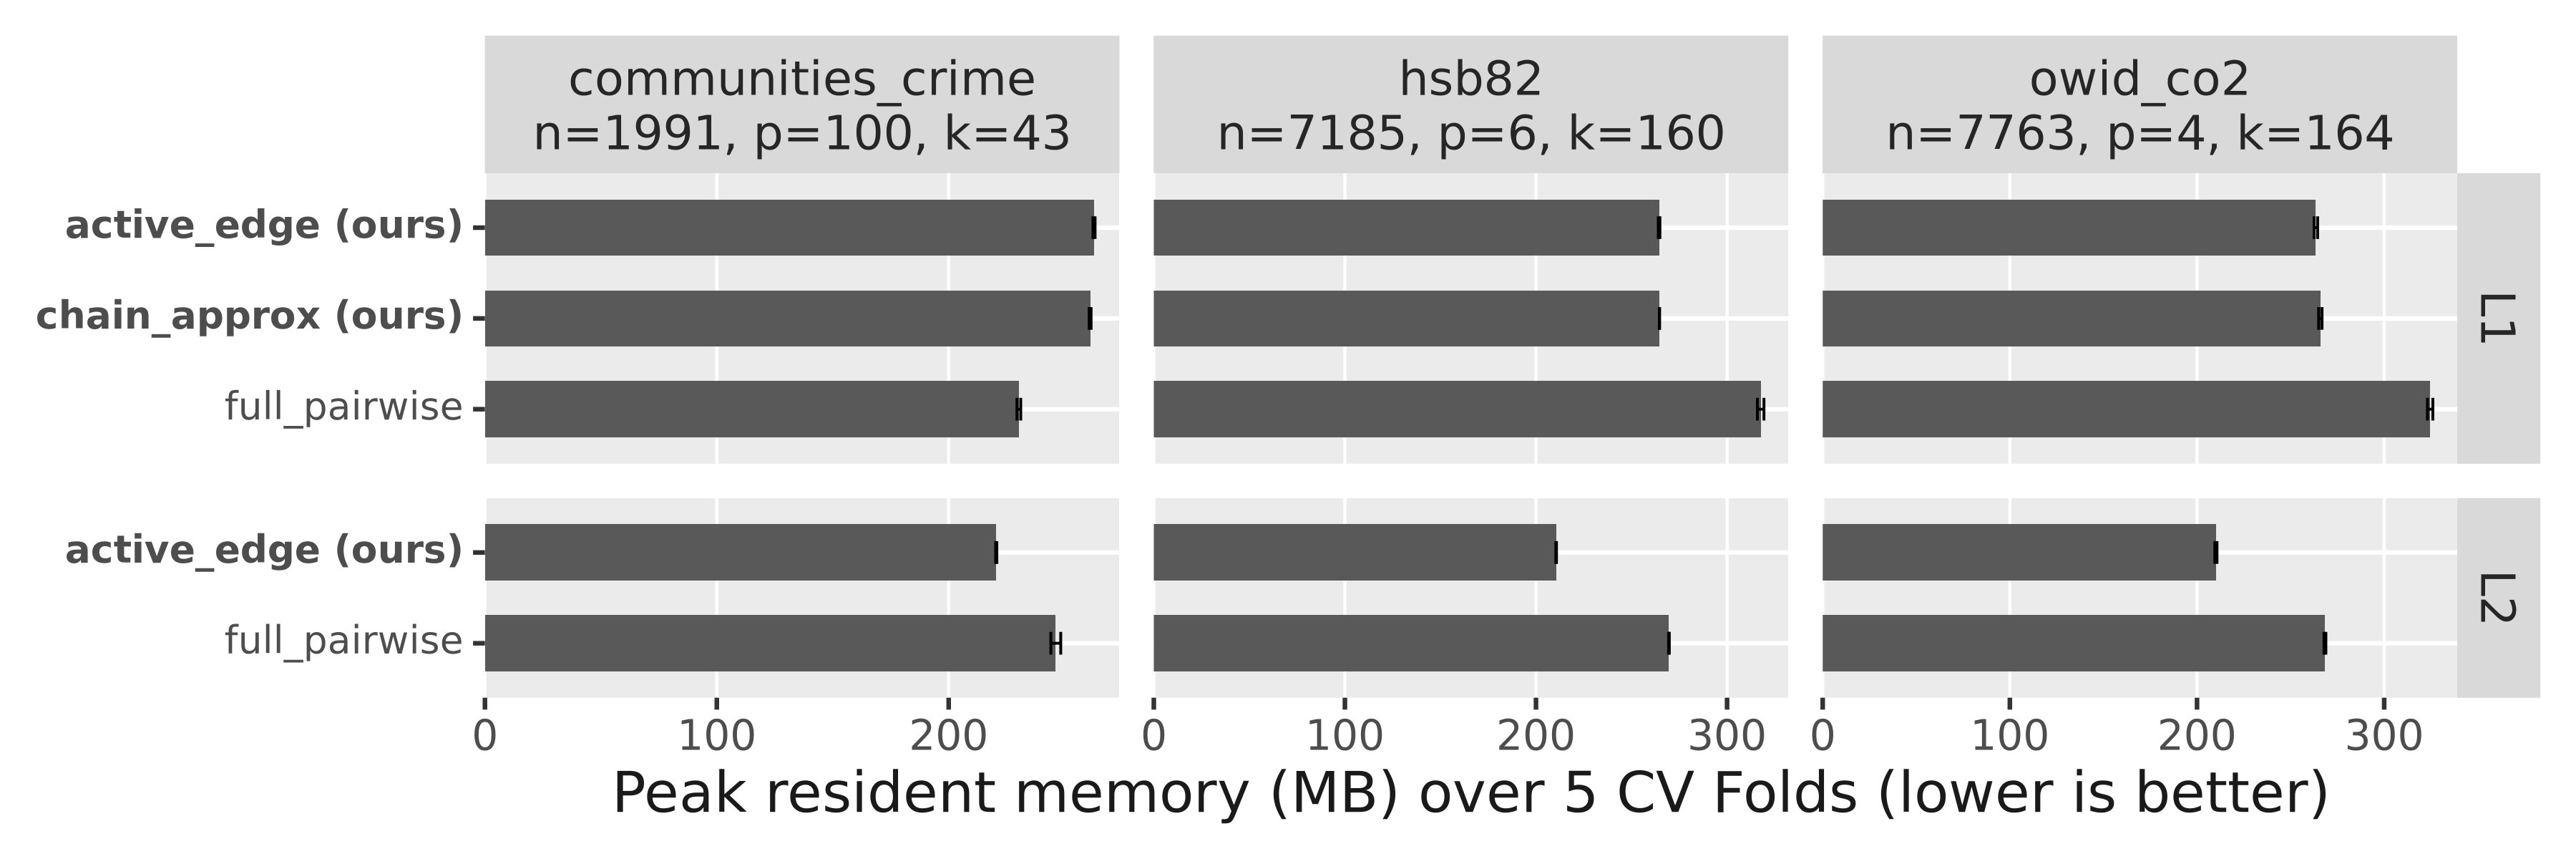
\includegraphics[width=\textwidth]{figures/hpc_l1_l2_three_datasets_memory.png}
  \caption{Peak resident memory for the same representative datasets and solver families shown in Figure~\ref{fig:l1-l2-accuracy-three-datasets}.
  Bars show mean peak resident set size in MB over five cross-validation folds, with error bars showing one standard deviation. 
  Lower values are better.}
  \label{fig:l1-l2-memory-three-datasets}
\end{figure}



\subsection{Runtime-Memory Efficiency Gains}
Figure~\ref{fig:l1-l2-pareto-gains} summarizes the exact L1 operator gains across the real data benchmark panel.
Each point compares the active-edge L1 operator with the full-edge L1 reference on the same dataset.
The horizontal coordinate is the log ratio of fit time, and the vertical coordinate is the log ratio of peak memory.  
Points to the left of zero are faster than the full-edge reference, points below zero use less memory, and points in the lower-left quadrant improve both.
Labels report the dataset, the number of groups, and the percent RMSE change relative to the full-edge reference.

The plot is interpreted as a standard multiobjective efficiency comparison, where methods are compared by accuracy and computational cost.
A method is preferable only if it improves one resource without worsening the other, or if the tradeoff is explicit. 
This is relevant because sparse-graph solvers are intended to reduce both arithmetic work and the amount of graph-derived state that must be kept in memory. 
The plot separates three empirical claims. 
First, the RMSE labels stay near zero, confirming that the operator representation preserves the fitted L1 objective. 
Second, most datasets move left, showing faster fitting. 
Third, many points also move downward, showing lower peak resident memory.
Points in the upper-left quadrant are still faster but use slightly more memory.

The two panels connect the separate timing and memory results. 
In the L1 panel in Figure~\ref{fig:l1-l2-pareto-gains}, most datasets move left, and many also move downward, but the memory gains are smaller and less uniform than the timing gains. 
The L2 panel is shifted farther left and mostly downward because active-edge augmented-design construction reduces both
the number of rows built before \texttt{glmnet} and the sparse objects held by the worker process. 
These patterns match the construction-cost analysis in Section~\ref{sec:solvers}.
Across the L1 and L2 benchmarks, peak resident memory ranged from about 70 MB for featureless fits to about 500 MB for the largest full-pairwise reference fit.

\begin{figure}[t]
  \centering
  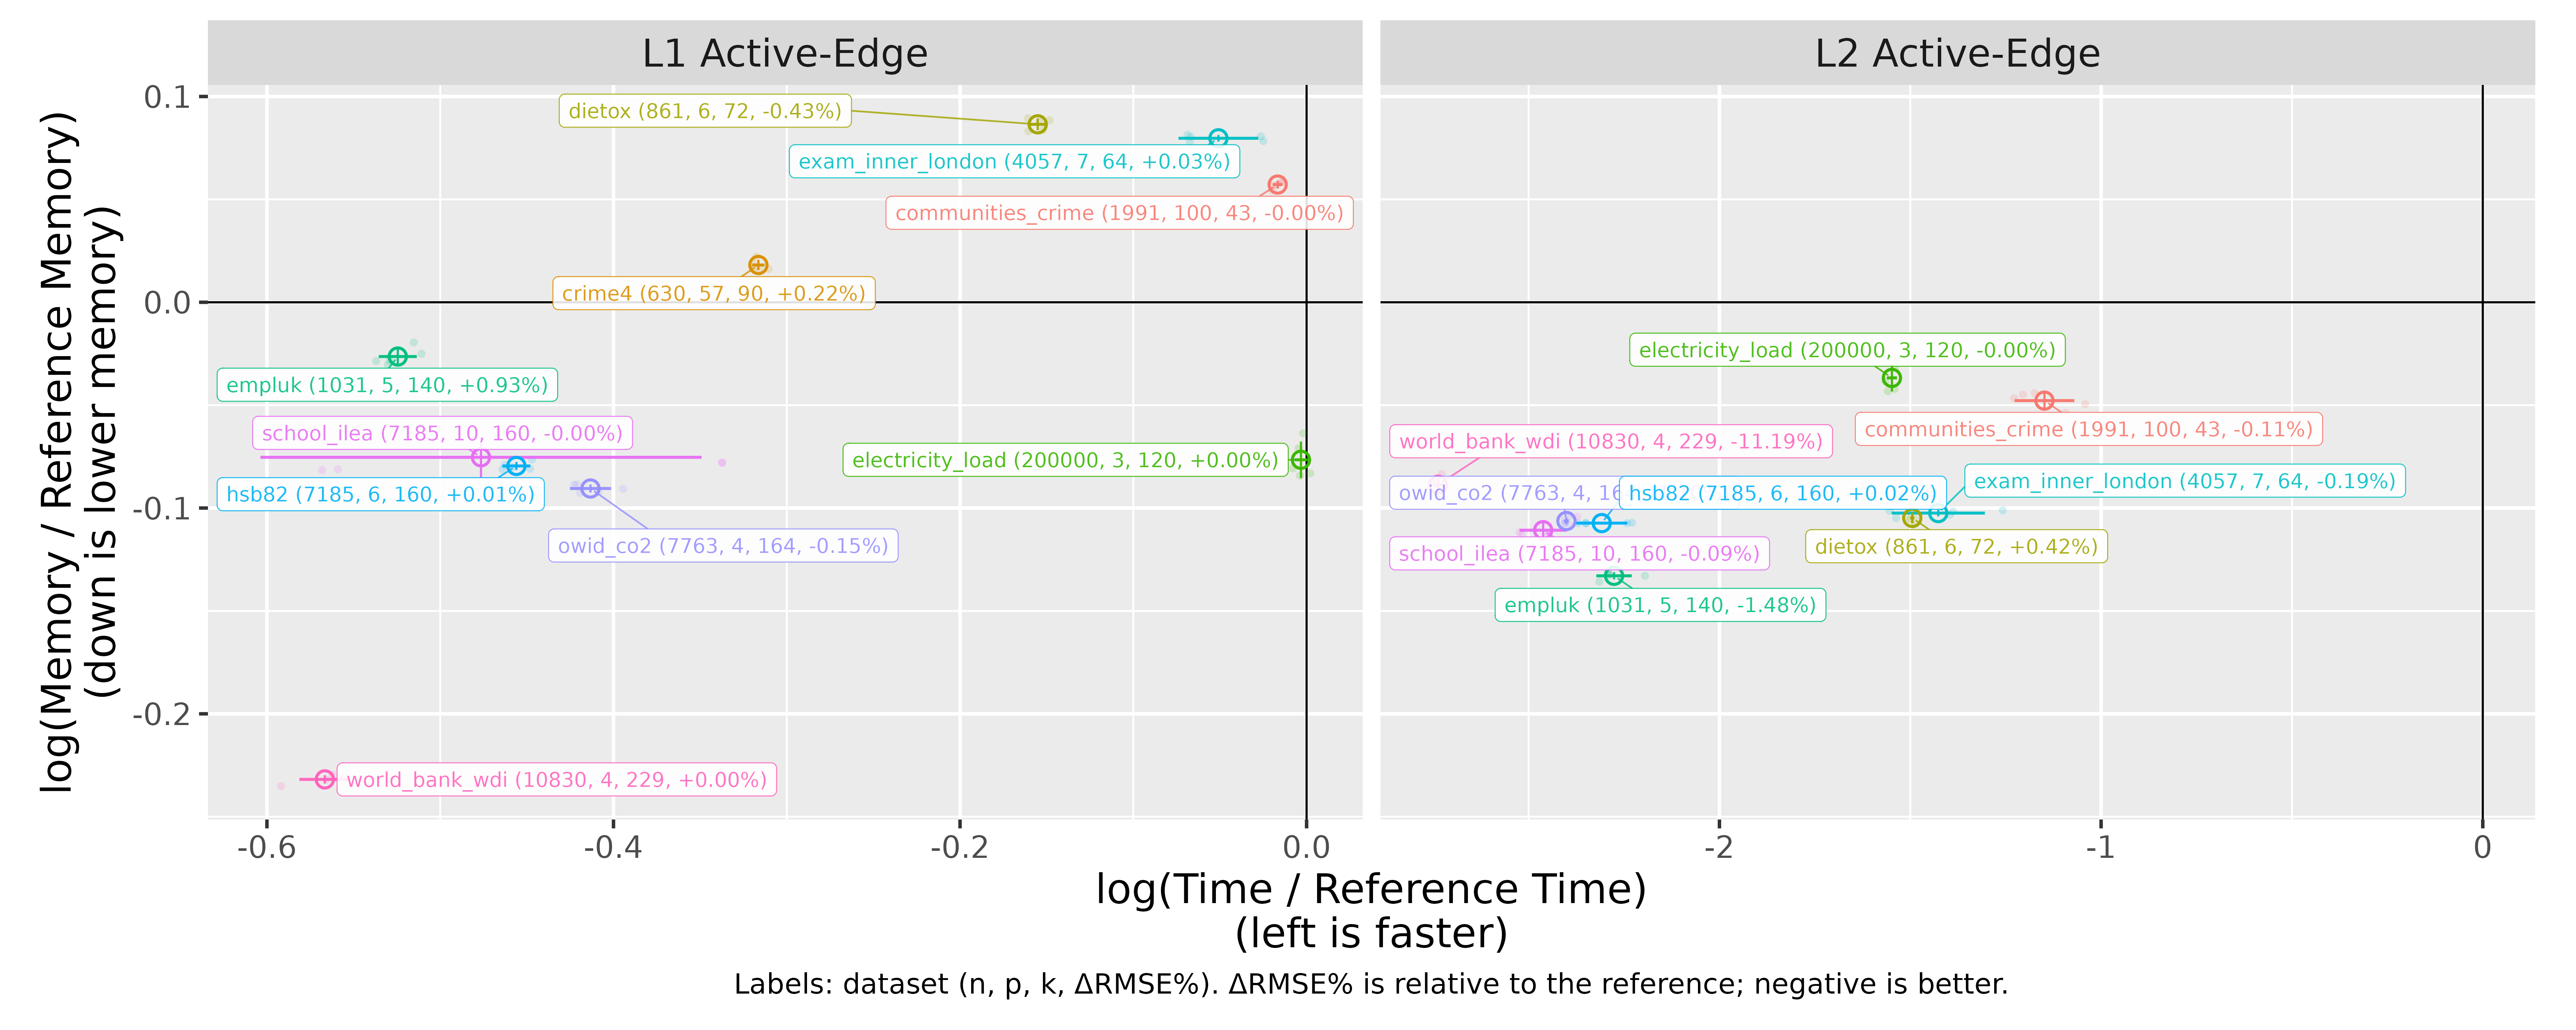
\includegraphics[width=\textwidth]{figures/hpc_l1_l2_combined_pareto.png}
  \caption{Runtime-memory Pareto plots for the exact active-edge solvers.
  The L1 panel compares the active-edge operator with the full-pairwise L1 reference, and the L2 panel compares active-edge augmented-design construction with the full-pairwise L2 reference. 
  Left is faster, down is lower peak memory, and the lower-left quadrant indicates improvement on both efficiency axes.}
  \label{fig:l1-l2-pareto-gains}
\end{figure}

% \subsection{L1 Runtime-Memory Efficiency Gains}
% Figure~\ref{fig:l1-pareto-gains} summarizes the exact L1 operator gains across the real data benchmark panel.
% Each point compares the active-edge L1 operator with the full-edge L1 reference on the same dataset.
% The horizontal coordinate is the log ratio of fit time, and the vertical coordinate is the log ratio of peak memory.  
% Points to the left of zero are faster than the full-edge reference, points below zero use less memory, and points in the lower-left quadrant improve both.
% Labels report the dataset, the number of groups, and the percent RMSE change relative to the full-edge reference.

% The plot is interpreted as a standard multiobjective efficiency comparison, where methods are compared by accuracy and computational cost.
% A method is preferable only if it improves one resource without worsening the other, or if the tradeoff is explicit. 
% This is relevant because sparse-graph solvers are intended to reduce both arithmetic work and the amount of graph-derived state that must be kept in memory. 
% In the L1 solver, the dense full-edge representation stores and applies candidate pair constraints that are inactive for a sparse graph, whereas the active-edge operator stores endpoint and weight vectors only for nonzero graph edges. 
% This directly reduces the working set for fusion differences and scatter updates. 

% The plot therefore separates three empirical claims. 
% First, the RMSE labels stay near zero, confirming that the operator representation preserves the fitted L1 objective. 
% Second, most datasets move left, showing faster fitting. 
% Third, many points also move downward, showing lower peak resident memory.
% Points in the upper-left quadrant are still faster but use slightly more memory.

% The memory gains are also expected to be smaller and less uniform than the runtime gains because peak resident memory measures the whole fitting process, not only the graph representation. 
% The active-edge solvers reduce the working set associated with graph construction, but the process still stores the design matrix,
% response, group indices, coefficient iterates and validation objects. 
% In addition, peak memory can be determined by temporary sparse-matrix triplets, edge buffers, or copies created during construction.
% Therefore, the expected memory improvement is strongest when graph objects dominate the working set, and weaker when fixed data and runtime overheads dominate.

% \begin{figure}[t]
%   \centering
%   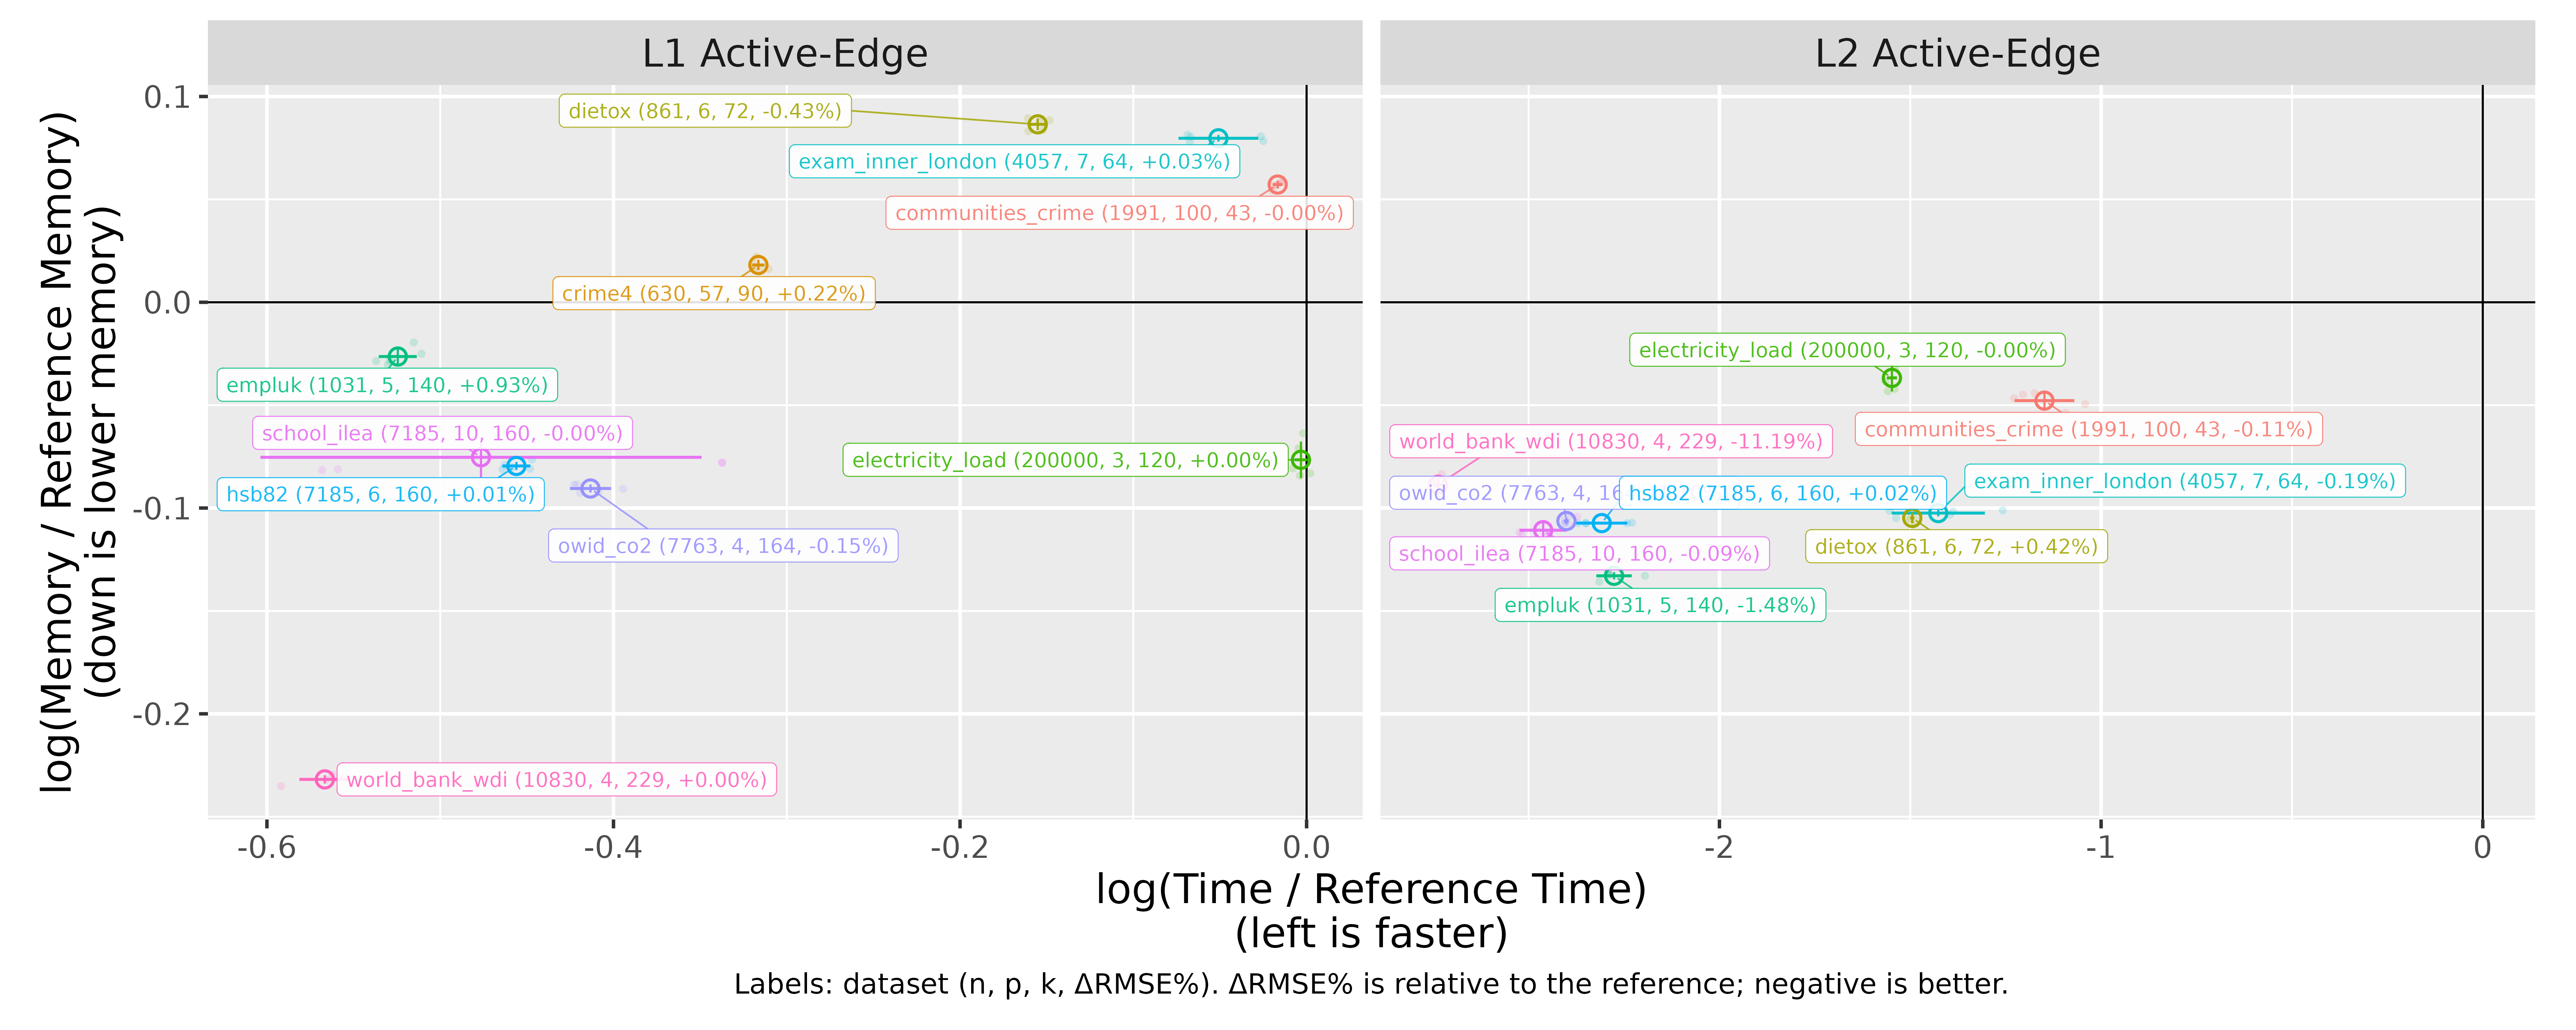
\includegraphics[width=1.0\textwidth]{figures/hpc_l1_l2_combined_pareto.png}
%   \caption{Runtime-memory plot for the exact L1 active-edge operator.
%   Each point compares the operator solver with the full-edge L1 reference on the same dataset. 
%   Left is faster, down is lower peak memory, and labels report dataset, number of groups, and percent RMSE change.
%   The lower-left quadrant indicates improvement on both efficiency axes.}
%   \label{fig:l1-pareto-gains}
% \end{figure}

% \subsection{L2 Runtime-Memory Efficiency Gains}

% Figure~\ref{fig:l2-pareto-gains} gives the corresponding efficiency plot for L2 fusion. 
% The active-edge L2 builder shows larger timing gains because the full-pairwise L2 reference first creates augmented regression rows for many group pairs that are absent from the sparse graph before passing the problem to \texttt{glmnet}. 
% When $k$ is large and the graph is sparse, deleting zero-weight pair rows changes the augmented design from an all-pairs construction to an active-edge construction with the same objective.

% Under full-pairwise construction, the fusion block contains $p_{\mathrm{eff}}\binom{k}{2}$ rows before zero-weight pairs are removed. 
% Under active-edge construction, the fusion block contains only $p_{\mathrm{eff}}m$ rows. 
% This changes the time required to build the augmented design, and also the number of sparse matrix entries, row indices, and intermediate triplets that must be held by the worker process. 
% The figure makes this visible because most datasets lie below zero on the memory axis, so active-edge L2 is faster and also reduces peak RAM demand.

% The L2 points are concentrated further to the left than the L1 points, which matches the construction cost analysis in Section~\ref{sec:solvers}.
% As in the L1 plot, the RMSE labels remain close to zero. 
% The larger downward and leftward shifts for high-$k$ datasets are the empirical signature of the sparse representation. 

% \begin{figure}[t]
%   \centering
%   
\includegraphics[width=.78\textwidth]{figures/hpc_l2_efficiency_diff_vs_old_l2_new_l2.png}
%   \caption{Runtime-memory plot for the L2 active-edge augmented-design builder. 
%   Each point compares active-edge construction with the full-pairwise L2 reference on the same dataset. 
%   Left is faster, down is lower peak memory, and labels report dataset, number of groups, and percent RMSE change.
%   The lower-left quadrant indicates improvement on both efficiency axes.
%   }
%   \label{fig:l2-pareto-gains}
% \end{figure}




\section{Discussion}

The experiments show that sparse fusion graphs need corresponding sparse computational representations. 
When the graph has $m$ edges, an implementation that constructs $O(k^2)$ pairwise constraints can lose the computational advantage of using a sparse graph. 
This is a general issue for edge-penalized regression. 
Any method whose penalty decomposes over graph edges can pay an unnecessary quadratic cost if the graph is represented by a complete set of candidate pairs. 
The L1 operator and L2 active-edge builders recover the intended $O(pm)$ fusion representation while preserving the original objective in the exact cases.

The exact L1 operator is the safest default among the proposed L1 solvers.
It preserves the same fitted objective as the reference active-edge formulation and gives substantial runtime and memory improvements. 
The chain-approximation solver is an approximation for exploratory or large-scale cases where a small loss in predictive accuracy is acceptable.

The solver representation aligns the computational graph with the modeling graph. 
Edge-explicit L1 fusion updates, blocked edge processing, DFS/MST chain approximation, and active-edge L2 matrix construction are instances of that representation. 
Proposition~\ref{prop:l1-convergence} gives the corresponding smoothed-objective convergence guarantee for the L1 APG updates, while Propositions~\ref{prop:l1-equivalence} and~\ref{prop:l2-equivalence} identify the exact cases where the new representations preserve the main objective.
Proposition~\ref{prop:complexity} clarifies how the graph construction cost changes with the number of represented edges.
The chain-approximation method is separated from those exact methods because replacing a graph by a chain changes the fusion geometry.
Proposition~\ref{prop:chain-target} states the precise chain objective being optimized and the omitted-edge penalty that accounts for the approximation.

The empirical evidence is strongest for the exact L1 operator and active-edge L2 construction. 
The chain method provides a more aggressive efficiency option, but it changes the fusion graph before fitting.
For sparse L1 fusion, the exact active-edge operator is therefore the preferred default, while chain-approximation fitting is best viewed as an option for exploratory or analyses with tight memory budgets.


\subsection{When Sparse-Graph Representations Help}
The sparse-graph representation is most useful when the modeling graph has far fewer active edges than the complete graph. 
The estimators considered in this paper allow arbitrary fusion graphs, including complete graphs. 
If the intended graph is complete, then $m=\binom{k}{2}$ and active-edge construction remains correct but does not reduce the asymptotic graph-representation cost.
The computational gains therefore come from settings where the graph encodes a structured notion of similarity, such as temporal adjacency, spatial neighborhoods, nearest-neighbor group similarity, or task relationships.
For complete or nearly complete graphs, the only L1 solver in this paper that can still reduce the fusion edge budget substantially is the chain approximation. 
It does so by replacing the original graph with a connected chain, so the gain comes from changing the optimization target rather than from an exact sparse representation of the same graph. 

This distinction is separate from the statistical question of which graph is best for prediction. 
A complete graph may be appropriate when all group pairs should be eligible for fusion. 
In contrast, sparse graphs are appropriate when domain knowledge or training-fold similarity suggests that only a limited set of group relationships should be penalized directly. 
The contribution of the active-edge solvers is to make this sparse modeling choice visible to the
optimizer. 


\subsection{Scope of the Optimization Comparisons}
The experiments compare the new representations against the reference grouped fused-regression solvers rather than against a broad collection of alternative optimizer families. 
This choice is central to the empirical design. 
The L1 reference solver and the exact active-edge operator both use the same smoothed proximal-gradient framework. 
The L2 reference and active-edge solvers both use the same augmented-design reduction followed by \texttt{glmnet}. 
The comparisons therefore hold fixed the statistical objective, graph, folds, hyperparameter selection, prediction pipeline, and optimizer family. 
The primary changing factor is the representation of the graph-fusion term. 
This isolation  makes the empirical results interpretable as evidence for the sparse-graph representation principle.

Alternative optimizers, including ADMM and split-Bregman methods, are important for fused-lasso problems and can be very effective in other settings. 
An ADMM formulation would typically introduce auxiliary variables for edge differences, enforce $z_{uv}=\beta_u-\beta_v$ with augmented-Lagrangian updates, alternate between coefficient, edge-variable, and dual updates, and require choices of penalty parameters and stopping rules. 
Such a comparison would mix representation effects with optimizer effects. 
Pre-conditioners, penalty-parameter tuning, convergence tolerances, warm starts and sparse-matrix backends could all influence runtime and memory.
Those factors would not isolate the question studied here.

This distinction also clarifies the role of the reference fused-lasso baseline.
It is included because it is the direct predecessor for the grouped fused-regression objective and software interface considered in this paper. 
Beating that baseline while preserving the same optimizer family shows that the gain comes from avoiding zero-weight all-pair graph construction rather than from replacing the optimization architecture. 
The same active-edge principle could be incorporated into ADMM or other edge-splitting methods, where the number of auxiliary edge variables and dual updates would also scale with the represented edge set. 
Developing and tuning such solvers is a separate algorithmic comparison and is left for future work.

There are two important limitations. 
First, the guarantees cover representation equivalence, smoothing error, convergence for the smoothed L1 objective, and graph-construction complexity. 
The statistical properties are those of the underlying fused-lasso and graph-guided regression objectives, while the contribution here is to preserve those objectives with a sparser computational representation. 
Second, the largest gains occur when the user-supplied or data-derived graph is sparse. 
If the modeling graph is close to complete, the active-edge representation has little to no advantage.

\section{Implementation Details}
The active-edge and chain approximation used for the sparse-graph
comparisons are implemented entirely in R programming language.
The main implementation challenge was to change the graph representation without changing the fitted objective. 
In the original all-pair construction, inactive graph pairs can still appear as zero-weight algebraic objects.
This implies, looping over edges that do not exist, essentially wasting resources.
Although, this is convenient for indexing, but it hides sparsity from the solver. 
The L1 operator code therefore first converts the fusion graph into edge arrays $(u_e,v_e,w_e)_{e=1}^m$ and keeps those arrays as the only fusion structure used inside the accelerated iterations. 
Each edge update computes a coefficient difference, clips the smoothed dual quantity, and scatters the result back to the two incident group columns with opposite signs. 
The difficult part was preserving the same orientation, weighting, intercept convention, group ordering, and final thresholding semantics as the reference implementation.

Memory management was another practical issue. 
A direct vectorized implementation can form a large edge by coefficient matrix during each L1
iteration. 
That is fast for moderate problems but can dominate memory when both $p$ and $m$ are large. 
The implementation supports blocked edge processing, which applies the same scatter updates in edge batches while keeping the accumulated gradient in the original coefficient matrix shape.
The chain solver required a separate step. 
Specifically, groups are temporarily reordered along the selected chain for fast adjacent differences and then reordered back before returning fitted coefficients.

The L2 implementation required a different construction. 
The statistical problem is represented as an augmented least-squares design passed to \texttt{glmnet}. 
The key coding step was to build this augmented matrix directly from sparse triplets. 
For each active edge $(g,h)$ and each fused coefficient coordinate, the builder emits one row with opposite signed entries in the two group blocks and a zero augmented response. 
This avoids allocating rows for inactive group pairs. 
The implementation also preserves the original loss scaling and lambda correction convention, so that any observed difference between full-pair and active-edge runs comes from the represented graph rows.

\section{Software Availability}

The algorithms are available in the open-source R package \texttt{sparsefusion} at \url{https://github.com/EngineerDanny/sparsefusion}. 
A grouped regression problem is supplied as a feature matrix $X$, response vector $y$, group labels \texttt{groups}, and a symmetric fusion graph matrix $G$.
For new data, the recommended entry point is \texttt{sparse\_fusion}. 
The argument \texttt{fusion} selects \texttt{l1} or \texttt{l2} fusion, and the argument \texttt{solver} selects \texttt{active\_edge}, \texttt{full\_pairwise}, or \texttt{chain\_approx}. 
The \texttt{active\_edge} solver is the exact sparse graph representation for L1 and L2 fusion, \texttt{full\_pairwise} runs the reference all-pair construction, and \texttt{chain\_approx} runs the approximate L1 chain solver.
For example, an exact sparse-graph L1 fit on new grouped data can be run as
follows:
\begin{verbatim}
library(sparsefusion)

fit <- sparse_fusion(
  X, y, groups, G,
  lambda = 1e-3,
  gamma = 1e-2,
  fusion = "l1",
  solver = "active_edge"
)
\end{verbatim}

The returned object from each fitting function is a coefficient matrix with one column per group, so prediction on new observations requires selecting the coefficient column associated with the observation's group. 
The package includes examples, benchmark scripts, and a minimal reviewer example in the
repository README. 
The paper experiments call the same package functions used for new data analysis, with fixed folds and graph construction scripts stored
in the repository.

\section{Conclusion}
This paper studied the computational representation of sparse fusion graphs in grouped fused regression. 
The main finding is that a sparse statistical graph should remain sparse inside the optimizer. 
For L1 fusion, the active-edge operator evaluates the same smoothed fusion gradient as the full-edge construction after zero-weight pairs are removed. 
For L2 fusion, the active-edge augmented design gives the same quadratic fusion objective while constructing rows only for nonzero graph edges. 
These exact representations change the dominant fusion cost from all-pairs construction to construction that scales with the represented edge set.
The empirical results support the same conclusion. 
The exact L1 and L2 active-edge solvers preserve predictive accuracy relative to the corresponding full-construction references while reducing fit time and, in many cases, peak memory. 
The chain approximation L1 solver gives an additional option when reducing the edge budget is more important than preserving the original graph exactly. 

Several future directions remain open. 
First, the same active-edge representation principle could be incorporated into other optimizer families, including ADMM and split-Bregman methods, where auxiliary variables and dual updates should also scale with the represented edge set. 
Second, adaptive graph construction and hyperparameter selection could be studied jointly with the sparse solver representation, since the statistical value and computational cost of fusion both depend on the chosen graph. 
Third, lower-level sparse matrix and compiled implementations could further separate the algorithmic savings from fixed runtime overheads. 
These directions would test how far the representation principle extends beyond the grouped fused-regression solvers considered here.
The algorithms used in this paper are implemented in the project repository at \url{https://github.com/EngineerDanny/sparsefusion}.

% \appendix
% \section{Supplementary Dataset Inventory}
% \label{sec:supp-datasets}

% Table~\ref{tab:datasets} lists the complete union of datasets that appear in
% the final L1 and L2 result summaries used by this paper. The
% \texttt{SubsetType} column reports the semantic unit defining the subgroups in
% the regression problem after preprocessing in this repository.

% \begin{table}[H]
% \centering
% \scriptsize
% \caption{Public grouped-regression datasets used in the reported real data
% benchmark panels. The columns report total observations $n$, feature count
% $p$, group count $k$, and semantic subgroup type after preprocessing in this
% repository.}
% \label{tab:datasets}
% \begin{tabular}{@{}>{\raggedright\arraybackslash}p{0.24\textwidth}rrr
% >{\raggedright\arraybackslash}p{0.14\textwidth}
% >{\raggedright\arraybackslash}p{0.21\textwidth}@{}}
% \toprule
% Dataset & $n$ & $p$ & $k$ & \texttt{SubsetType} & Source \\
% \midrule
% \path{communities_crime} & 1,991 & 100 & 43 & states &
% UCI Communities and Crime \citep{uci_communities} \\
% \path{electricity_load} & 200,000 & 3 & 120 & meters &
% UCI Electricity Load \citep{uci_electricity} \\
% \path{owid_co2} & 7,763 & 4 & 164 & countries &
% Our World in Data CO2 \citep{owidco2} \\
% \path{rdatasets_crime4} & 630 & 57 & 90 & counties &
% Panel crime data \citep{cornwell1994crime} \\
% \path{rdatasets_dietox} & 861 & 6 & 72 &
% pigs & Dietox pig-growth data \citep{lauridsen1999dietox} \\
% \path{rdatasets_empluk} & 1,031 & 5 & 140 & firms &
% Employment panel data \citep{arellano1991panel} \\
% \path{rdatasets_exam_inner_london} & 4,057 & 7 & 64 &
% schools & Inner London exam data \citep{goldstein1993exam} \\
% \path{rdatasets_hsb82} & 7,185 & 6 & 160 & schools &
% High-school multilevel data \citep{raudenbush2002hlm} \\
% \path{school_ilea} & 7,185 & 10 & 160 & schools &
% \texttt{nlme} school data \citep{pinheiro2000mixed} \\
% \path{world_bank_wdi} & 10,830 & 4 & 229 & economies &
% World Development Indicators \citep{worldbankwdi} \\
% \bottomrule
% \end{tabular}
% \end{table}


\acks{
The author thanks the maintainers of the public datasets and R packages used in the empirical evaluation. 
The authors also acknowledge Northern Arizona University's high-performance computing resources for supporting the computational experiments. 
This work was supported by National Science Foundation award 2125088 through the Rules of Life program. 
Any opinions, findings, and conclusions or recommendations expressed in this material are those of the author and do not necessarily reflect the views of the National Science Foundation.
}

\bibliography{refs}

\end{document}
